\documentclass[a4paper]{article}
\usepackage{pgfplotstable}
\usepackage{longtable}
\usepackage{varwidth}
\usepackage{array}
\usepackage{lscape}
\usepackage[top=4.5 cm,bottom=2.54cm, lmargin=2cm, rmargin=1.74cm, headheight=3.25cm]{geometry}
\usepackage{helvet}
\usepackage{tabto}
\usepackage{collcell}
\usepackage{seqsplit}
\usepackage{fancyhdr}
\usepackage{lastpage}
\usepackage{xcolor}
\usepackage{sectsty}
\usepackage{mdframed}
\usepackage{draftwatermark}
\usepackage{textpos}
\usepackage{placeins}
\usepackage{listings}
\usepackage{tikz}
\usepackage[hidelinks]{hyperref}

\SetWatermarkText{Draft}

\definecolor{maroon}{RGB}{102,0,33}
\sectionfont{\color{maroon}}  % sets colour of section headings

\renewcommand{\familydefault}{\sfdefault}

% Set title etc
\title {Copernicus Climate Change Service - 311a Lot 2 \\ Defining a Common Data Model}
\author {David I. Berry \\ National Oceanography Centre, UK}
\date{\today}

% empty header style for tables later on
\pgfplotstableset{
empty header/.style={
           typeset cell/.append code={%
               \ifnum\pgfplotstablerow=-1 %
                   \pgfkeyssetvalue{/pgfplots/table/@cell content}{}%
               \fi
           }
       }
   }

% new column for tables to split long strings
\newcolumntype{n}[1]{  > {\collectcell\seqsplit} V{#1} < {\endcollectcell}    }

% no indent of new paragraphs
\setlength{\parindent}{0pt}

% framed text boxes
\newcounter{FramedDepth}
\setcounter{FramedDepth}{-1}
\mdfdefinestyle{Framed}{linecolor=black,linewidth=1pt,leftmargin=10pt,rightmargin=10pt,
                        innerleftmargin=10pt,innerrightmargin=10pt}
\newenvironment{Framed}{%
  \addtocounter{FramedDepth}{1}
  \ifcase\theFramedDepth\def\FrameColour{white!50}%
    \or\def\FrameColour{white!50}%
    \or\def\FrameColour{white!50}%
    \or\def\FrameColour{white!50}%
    \fi%
  \begin{mdframed}[style=Framed,backgroundcolor=\FrameColour]%
}{\end{mdframed}\addtocounter{FramedDepth}{-1}}


% 1.25 18.4, 1.7
% 0.65
% Copernicus logo on page 3 onwards needs to go at (18.4cm, 1.7cm from top left of page) size (0.9cm by 0.86 cm)

% headers and footers
\headheight 3.5 cm          
\headsep  0.5 cm

\lhead{\textcolor{maroon}{Copernicus Climate Change Service}\vskip 0.5 cm}
\rhead{\includegraphics{/Users/dyb/GitHub/common_data_model/png/c3s_logo_small.png} \vskip 0.3 cm}

\lfoot{C3S\_311a\_Lot2\_NUIM\_2017 \{ref\} }
\cfoot{}
\rfoot{Page \textbf{\thepage}  of \textbf{\pageref{LastPage}} }

\pagestyle{fancy}

\begin{document}\thispagestyle{empty}


% Cover sheet

% top banner
\begin{tikzpicture}[remember picture,overlay]
\draw ([yshift=-15.7mm]current page.north) node[inner sep=0] (a) {\includegraphics[width=\paperwidth]{/Users/dyb/GitHub/common_data_model/png/c3s_banner_top.png}};
\draw ([yshift=-25.7mm]current page.north) node[inner sep=0] (a) {
\includegraphics[width=62.8mm]{/Users/dyb/GitHub/common_data_model/png/copernicus_logo_large.png}};
\node[shift={(0 mm, -10mm)}]  at (current page.north)   {
\tiny\color{white} ECMWF COPERNICUS REPORT \\
};
\end{tikzpicture}

% top maroon bar
\begin{tikzpicture}[remember picture,overlay]
\draw ([yshift=-53.3 mm]current page.north) node[inner sep=0] (a) {
\includegraphics[width=\paperwidth]{/Users/dyb/GitHub/common_data_model/png/header_bar.png}};
\draw ([xshift=95mm, yshift=-53.0 mm]current page.north) node[inner sep=0] (a) {
\includegraphics[width=11.8mm]{/Users/dyb/GitHub/common_data_model/png/logo_thermometer.png}};
\draw ([xshift=89mm, yshift=-55.0 mm]current page.north) node[inner sep=0] (a) {
\includegraphics[width=12.0mm]{/Users/dyb/GitHub/common_data_model/png/logo_earth.png}};
\node at (1.5,-0.15)   {
    \color{white} Copernicus Climate Change Service
};
\node at (2.5,-0.65)   {
    \color{white} Copernicus Climate Change Service
};
\end{tikzpicture}


\vskip 4cm
\begin{center} 
\Large\textbf{Copernicus Climate Change Service - 311a Lot 2 \\ Defining a Common Data Model}
\vskip 1cm
\Large C3S\_311a\_Lot2\_NUIM - Access to Observations from Global Climate Data Archives
\end{center}

%footer bar
\begin{tikzpicture}[remember picture,overlay]
\draw ([yshift=15. mm]current page.south) node[inner sep=0] (a) {
\includegraphics[width=\paperwidth]{/Users/dyb/GitHub/common_data_model/png/footer_bar.png}};
\draw ([yshift=10.5 mm]current page.south) node[inner sep=0] (a) {\includegraphics{/Users/dyb/GitHub/common_data_model/png/copernicus_logo.png}};
\draw ([xshift=-30 mm, yshift=10.5 mm]current page.south east) node[inner sep=0] (a) {\includegraphics{/Users/dyb/GitHub/common_data_model/png/ECMWF_logo.png}};
\draw ([xshift=30 mm, yshift=10.5 mm]current page.south west) node[inner sep=0] (a) {\includegraphics{/Users/dyb/GitHub/common_data_model/png/ec_logo_small.png}};
\end{tikzpicture}
\newpage

\vspace*{\fill}
\begin{Framed}
This document has been produced in the context of the Copernicus Climate Change Service (C3S).\\
The activities leading to these results have been contracted by the European Centre for Medium-Range Weather Forecasts, operator of C3S on behalf of the European Union (Delegation Agreement signed on 11/11/2014). All information in this document is provided "as is" and no guarantee or warranty is given that the information is fit for any particular purpose.\\
The user thereof uses the information at its sole risk and liability. For the avoidance of all doubts, the European Commission
and the European Centre for Medium-Range Weather Forecasts has no liability in respect of this document, which is merely representing the authors view.
\end{Framed}

% title page
\newpage

\maketitle

\vskip 0.25in
\section*{Summary}
\hrule
\vskip 0.25in
This document describes background information on the definition of a common data model for the representation of in situ observations as part of the C3S 311a activity.\\ \\
A draft data model is proposed.\\ \\
\textbf{Call participants are requested to}:\\
\begin{itemize}
\item Review the proposed data model, specifically tables 3 - 7.
\item Review the configuration field tables and suggest modifications, additions and deletions.
\item Review the configuration code tables and suggest modifications, additions and deletions.
\item Review the code tables and propose / identify where an existing table (e.g. BUFR code table) and be used in replacement.
\end{itemize}
\vskip 0.25in
Tab separated versions of the code tables can be found at:\\ \\
\tabto{2cm} \url{https://github.com/glamod/common_data_model/tree/master/tables}
\vskip 0.25in
\hrule

\newpage
\tableofcontents
\newpage
\listoftables
\newpage


\section {Introduction}

\subsection {Purpose of this document}
This document defines the initial version of the Common Data Model (CDM)\footnote{As noted in the ITT: A common data model is different from a file format, which defines how information is encoded in a file. The purpose of a data model is to provide a well-defined data structure that can be used to represent data records from a variety of sources, in such a way that the information contained in those records can be unambiguously accessed using a common set of tools. Development of a common data model for observations involves specification of data attributes and their symbolic names, including, for example, identifiers for different instruments, observed parameters, geolocation and timing, etc. A governance structure is required to manage such specifications, ensure consistency with standards where they exist, and to ensure a controlled evolution of the data model.} developed within the Copernicus Climate Change Service (C3S) Access to Global Land and Marine Observations Database (C3S 311a Lot 2) service. This has been developed in consultation across the C3S 311a (Collection and Processing of In Situ Observations) Lots and ECMWF.

\subsection {Scope}
The defined common data model is intended for use with in situ land and marine observations. Instantaneous (or point) observations and temporal statistics (e.g. daily and monthly min / max temperatures, accumulation of precipitation etc.)  are supported through the use of a significance qualifier. Similarly, profile data is supported through reporting the z-coordinate alongside the observed value.\\

Whilst initially intended for use with observations of Essential Climate Variables (ECVs; e.g. GCOS, 2010) the data model is not restricted to the ECVs. Following the ECMWF Observations DataBase (ODB) type data model, the observand is parameterized, with both the variable being reported and it's value specified in the data model.\\

Comprehensive metadata is supported through the use of configuration tables, recording information on:
\begin{itemize}
\item Source level metadata: e.g. original source of data, source data centre, citation information etc.
\item Station level metadata: e.g. location, operating institute, parameters reported etc.
\item Profile level metadata: Additional information for profile data, e.g. unwinder type, type of balloon or XBT etc.
\item Sensor level metadata: e.g. calibration history and status, sensor type / serial number etc.
\end{itemize}
Comprehensive quality control and uncertainty information can be record through the use of linked entity-attribute-value tables.

\subsection {Structure of this document}

Section 2 of this document provides backgound information on the data model and existing relevant data models and standards. Section 3 forms the core section of this document and defines the primary observations table and associated configuration, quality control and uncertainty budget tables. Recognising that the data model will change and evolve as the requirements of the users and the C3S Climate Data Store develop, Section 4 proposes a goverance model for the CDM and outlines future developments.

\section {Background and existing standards}
\subsection {Observational sources and requirements of the data model}

Across the C3S 311a (Collection and Processing of In Situ Observations) service access to observations from the surface terrestrial and marine environments and upper air data will be provided in a Common Data Model. The observations included in the service range from point observations made from moving platforms to daily and monthly statistics at fixed locations.  The parameters reported include, inter alia: air temperature; humidity; wind speed; pressure; cloud cover information; present weather. The statistics include, inter alia: daily min, max and mean air temperature; accumulated precipitation over 3 or 24 hours; mean wind speed over the preceding 10 minutes. The full range of parameters and statistics to be reported will evolve as the service is developed. As new parameters are recovered from newly digitised sources and the reprocessed climate archives the list of parameters will need to expand.\\

Both surface level (terrestrial and marine) and upper air data will be included in the service.  The surface level data includes observations made at standard and non-standard heights. The upper air data will include multiple observations, starting at the surface and at increasing height through the atmosphere, often as a function of pressure or geopotential height. As a result the data model needs to include the flexibility to record the height and the units used for reporting the height of observation with every observation. Similarly, some reporting stations, and hence observations, will move in the horizontal plan, and the horizontal coordinates need to be reported with each observation. To avoid ambiguity, the CRS should be provided with each location reported.\\

The period covered by the service ranges from $\sim$1850 to present day. Over this period there have been many changes to the instruments and practices used to record the various parameters. The choice of instruments and practices will influence the quality of the observations and a change in instrumentation, or location, may introduce inhomogeneities into the record.  To mitigate this risk, comprehensive observational metadata, where it exists, is required. Similarly, information on adjustments and conversions applied to the data need to be recorded. The full range of observational practices and instruments used is not currently known and developed data model will need to be expandable to accommodate new metadata as required.\\

The observations to be included will be sourced from a variety of existing datasets, such as the International Comprehensive Ocean and Atmosphere Data Set (ICOADS; e.g. Freeman et al., 2017), and newly digitised sources. In defining the data model the provenance and lineage of the data sources need to be preserved. Similarly, usage rights and citation information for those data sources need to be preserved and provided to the users alongside the observational data.\\

In order to meet the above requirements a data model based on the ECMWF Observations DataBase (ODB) model has been developed, with the use of linked tables providing information on the observational and provenance metadata. The ODB type model allows for expansion to new parameters through the use of a parameterized observation list (see next section). The linked tables will define a core set of parameters under 4 different categories (station, source, profile and sensor), flexibility will be provided through the specification of optional elements and associated decode tables.\\

\subsection{ECMWF Observations DataBase (ODB)}

The data model defined and used in the ECMWF Observations DataBase (ODB) software allows the representation of environmental data from many sources, including in situ observations, satellite data and model output. This flexibility is achieved through storing each observation, or estimate, of a single parameter as a separate record together with header information providing information on the location and source of the observation. Where multiple observations are made in a single report the report spans multiple records, with the header information repeated. A simplified example is given in Table 1.\\

\pgfplotstabletypeset[
   empty header,
    begin table=\begin{longtable},
    %every head row/.style={output empty row},
    every nth row={1}{before row=\hline},
    every first row/.append style={
        before row={%
            % Initial caption
            \caption{Simplified example of records in ODB type data model, with observations from reports 1 and 2 spanning multiple records. For simplicity, the z coordinate has been omitted but profile data would be represented with each layer / height as a separate record}
            \label{tab:DataTableODB}\\
            % Initial column headers
            \hline\hline
            \multicolumn{5} {c} { \textbf{header information}} & 
            \multicolumn{3} {c} { \textbf{observation information}} 
            \\
            \hline
            \multicolumn{1} { > {\centering}V{0.3 in}} { \textbf{record id}} & 
            \multicolumn{1} { > {\centering}V{0.3 in}} { \textbf{report id}} & 
            \multicolumn{1} { > {\centering}V{0.3 in}} { \textbf{obs id}} & 
            \multicolumn{1} { > {\centering}V{1 in}} { \textbf{date}} & 
            \multicolumn{1} { > {\centering}V{1 in}} { \textbf{location}} & 
            \multicolumn{1} { > {\centering}V{0.75 in}} { \textbf{parameter}} & 
            \multicolumn{1} { > {\centering} V{0.75 in} } {\textbf{value}} &
            \multicolumn{1} { > {\centering} V{0.75 in} } {\textbf{units}} 
            \\ \hline\hline \endfirsthead
            \multicolumn{6}{c}{Table \thetable\ adjustment (cont.)} \\
            % column headers on additional pages
            \hline\hline 
            \multicolumn{5} { > {\centering}V{2.9 in}} { \textbf{header information}} & 
            \multicolumn{3} { > {\centering}V{2.25 in}} { \textbf{observation information}} 
            \\
            \hline
            \multicolumn{1} { > {\centering}V{0.3 in}} { \textbf{record id}} & 
            \multicolumn{1} { > {\centering}V{0.3 in}} { \textbf{report id}} & 
            \multicolumn{1} { > {\centering}V{0.3 in}} { \textbf{obs id}} & 
            \multicolumn{1} { > {\centering}V{1 in}} { \textbf{date}} & 
            \multicolumn{1} { > {\centering}V{1 in}} { \textbf{location}} & 
            \multicolumn{1} { > {\centering}V{0.75 in}} { \textbf{parameter}} & 
            \multicolumn{1} { > {\centering} V{0.75 in} } {\textbf{value}} &
            \multicolumn{1} { > {\centering} V{0.75 in} } {\textbf{units}} 
            \\ \hline\hline \endhead
            % Footer on 1st to penultimate pages
            \multicolumn{6}{r}{{Continued on next page}} \\
            \endfoot
            % Footer on last page of table
            \hline
            \multicolumn{6}{r}{{End of table}} \\ 
            \endlastfoot
        }
    },
    %
    end table=\end{longtable},
    col sep = &,
    row sep = \\ , 
    columns/record id/.style={string type, column type = V{0.3 in}},
    columns/report id/.style={string type, column type = V{0.3 in}},
    columns/observation id/.style={string type, column type = V{0.3 in}},
    columns/date/.style={string type, column type = V{1 in}},
    columns/location/.style={string type, column type = V{1 in}}, 
    columns/parameter/.style={string type, column type = V{1 in}},
    columns/value/.style={string type, column type = V{0.3 in}},
    columns/units/.style={string type, column type = V{0.3 in}}
]{
record id& report id& observation id& date & location & parameter & value & units \\
1 & 1 & 1 & 2012-01-01 12:00+0.0 & POINT(-40 40) & air temperature & 300.0 & K \\
2 & 1 & 2 & 2012-01-01 12:00+0.0 & POINT(-40 40) & sea level pressure & 1013.0 & hPa \\
3 & 2 & 3 & 2012-01-01 18:00+0.0 & POINT(-40.1 40.2) & air temperature & 300.3 & K \\
4 & 2 & 4 & 2012-01-01 18:00+0.0 & POINT(-40.1 40.2) & sea level pressure & 1013.2 & hPa \\
}


\subsection {BUFR and WIGOS Metadata Standard}
There has been a large body of work and significant effort previously invested in defining data models and parameterising the data and metadata for encoding the data into those data models.  Within the scope of the CDM and the C3S 311a service, the WMO Binary Universal Form for the Representation of meteorological data (BUFR) (WMO, 2015a) and the WMO Integrated Observing System Metadata Standard (WMDS) (WMO, 2015b) are key background material. \\

The BUFR format is a flexible and efficient table driven format for reporting weather observations on the WMO Global Telecommunications System (GTS) in binary. The tables defined as part of the BUFR format include many of the parameters that will be included in the CDM. For example, Common code table C6 (WMO 2015a) includes all the measurement units reportable in BUFR (and other WMO codes). Similarly, code tables are defined for reporting instrument types and methods, station types etc. Where possible, these code tables should be referenced and used in preference to defining new code tables.\\

In recognition of the increasing importance of observational metadata the WMDS is currently under development and undergoing a phased implementation (WMO, 2015b). The WMDS forms an extension of the ISO19115 metadata standard, with additional mandatory elements describing both the station level and discovery metadata as well as specific information on the instrumentation used and processing steps. As part of the process simplified versions of BUFR and other tables have been included in the standard. As with BUFR these tables should be referenced, where appropriate, in preference to defining new code tables. \\

\section {Common Data Model}
\FloatBarrier
Whilst the ODB data model has great flexibility the requirements of the implementation at ECMWF and that required by the C3S 311a service are different. For example, the existing columns defined within ECMWFs ODB implementation\footnote{http://apps.ecmwf.int/odbgov/column/}  contain many parameters that are of little relevance to the in situ observations but are relevant to the assimilation of data from many different sources into the numerical models. Conversely, there are many parameters included in the data from the C3S 311a service that are required to correctly interpret the observations but that are not included in ODB. \\

To give the flexibility required, and to maintain compatibility with the ODB, the primary observations table within the CDM has been developed based on the ODB model, but with the metadata linked / nested through a series of auxiliary / configuration tables. A schematic of this is shown in Figure 1 - a more complete schematic can be found at \url{https://github.com/glamod/common_data_model/blob/master/cdm_short.pdf}. In essence, the CDM constists of 7 primary tables:\\
\begin{itemize}
\item \textit{observations\_table} table (Table 2). This is the primary table, or data structure, containing the observations and the information on the geospatial location of the observations (and station), date / time of the report, the observed parameter, source information; data licensing and usage permissions etc and links to additional metadata.
\item \textit{station\_configuration} table (Table 3). This table contains detailed information on the station reporting the data including: institute operating the station; the type of station; station / AWS model type; location; operating territory; reporting frequency etc.
\item \textit{source\_configuration} table (Table 5). This table contains detailed information on the source dataset, including: information on the product; whether any processing has been applied; the original data centre the data were sourced from; citation information; the data licence for the product; how to cite the data source etc.
\item \textit{profile\_configuration} table (Table 7). This table contains detailed metadata for atmospheric and oceanic profiles, including: profile type; type of launcher; direction of profile; balloon / XBT type etc.
\item \textit{sensor\_configuration} table (Table 9). This table contains detailed information on the sensor used to make a particular observation, including: calibration status; sampling strategy; observing method; sensor housing and ventilation; instrument model and serial number etc.
\item \textit{qc\_table} table (Table 11). This table contains detailed information on the quality control applied to each report and / or observation.
\item \textit{uncertainty\_table} table (Table 13). This table contains detailed information on the uncertainty budget for each observation.
\end{itemize}

\begin{figure}
\centering
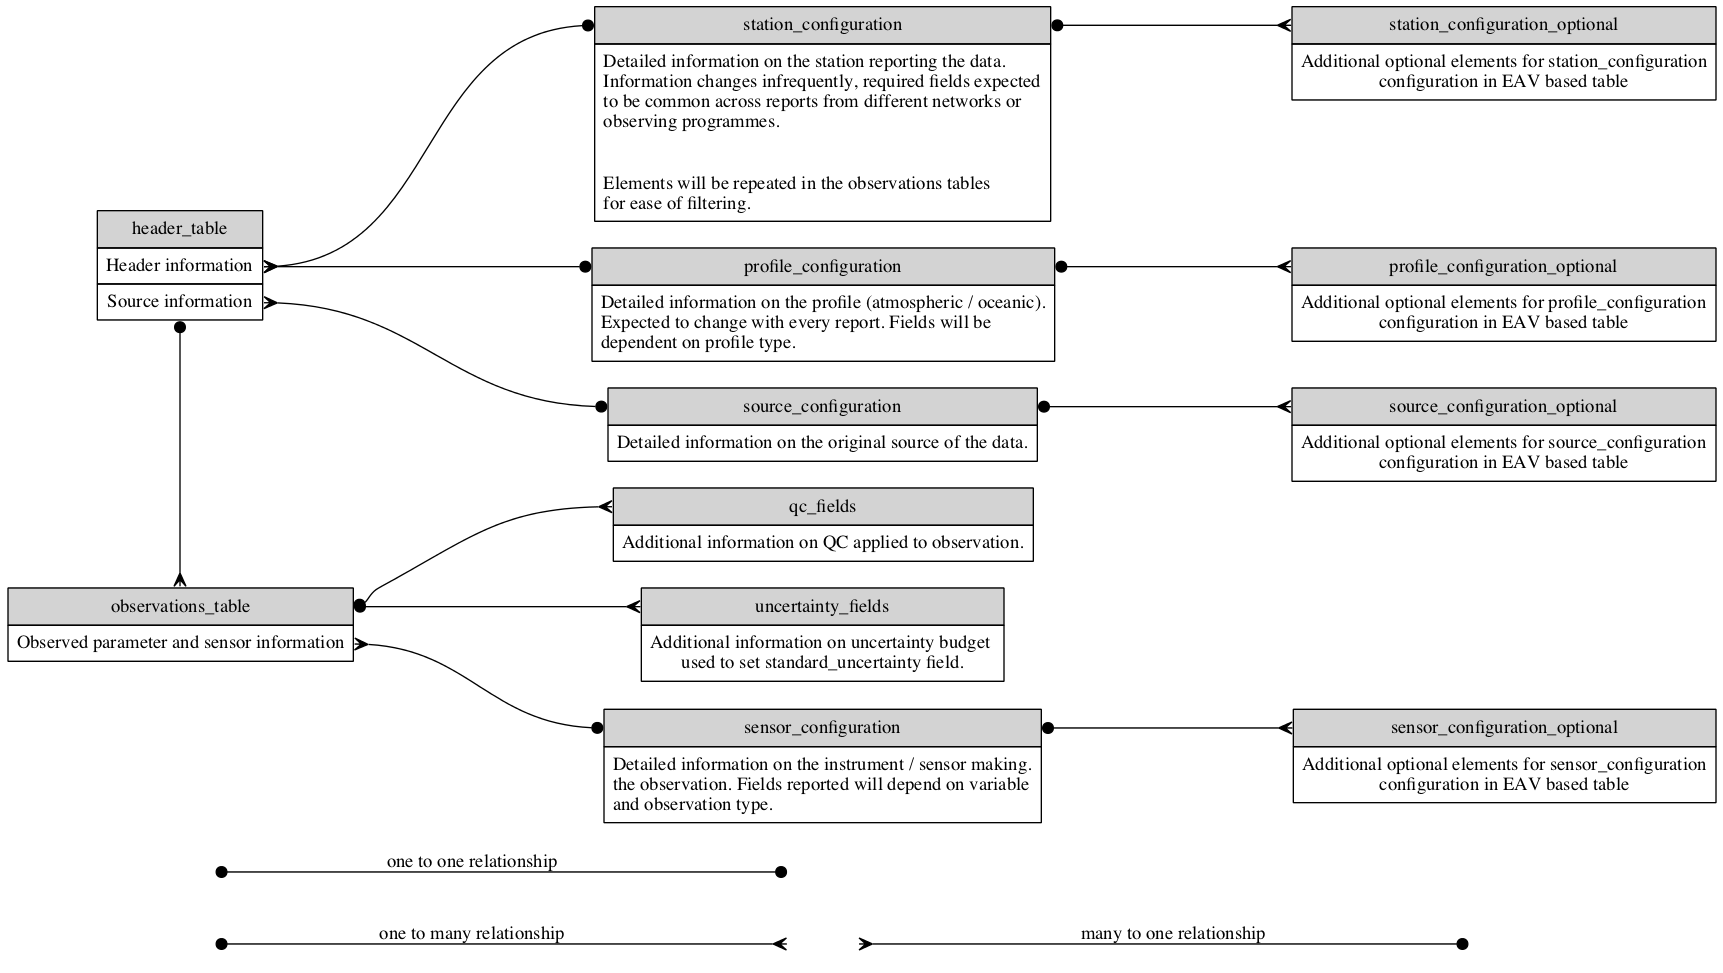
\includegraphics[width=1\textwidth]{/Users/dyb/GitHub/common_data_model/png/cdm_schematic_simple.png}
\caption {Simplified schematic showing overview of common data model}
\end{figure}

\FloatBarrier

Whilst Figure 1 and the tables show the data model from a relational database perspective the same data model could be represented in XML. A simplified XML example of this is shown in Figure 2. For readability the majority of elements have been omitted, with a few example elements and nested data structures retained. In this example, the records from the configuration tables are nested within the entries for the respective records from the observations\_table.\\

Within the following tables the following syntax has been used to indicate the data type for the different elements: \\
\begin{itemize}
\item numeric: \tabto{3 cm} Any numeric value (integer or floating point).
\item int: \tabto{3 cm} An integer value.
\item varchar: \tabto{3 cm} A variable length character string.
\item timestamp: \tabto{3 cm} A timestamp, e.g. "2017-07-01 00:00:0.0+00".
\item byte: \tabto{3 cm} A single byte of data used to store e.g. a bit flag array. 
\item {[]}:\tabto{3 cm} An array of the indicated type.
\item (fk)  \tabto{3 cm} The indicated value is also a foreign key linking to another table (e.g. encoded data and decode table).
\end {itemize}

Mandatory elements are indicated by a 1 (or 1+) in the occurance column. Mandatory elements that are not available must be encoded but may be reported as missing (.e.g NA or NULL). Optional elements are indicated by 0+. Whilst arrays have been indicated for the elements containing multiple values this does not preclude other implementations. Where there are many optional elements for a given table these are parameterised and included in the appendix. For example, the \textit{station\_configuration} table has many optional elements, with valid elements (and there kind / type) listed in the \textit{station\_configuration\_fields} table.

\begin{figure}
\begin{Framed}
\begin{lstlisting}[language=XML]
<observations_table>
    <report>
        <report_id type="integer"/>
        <region type="integer"/>
        <sub_region type="integer"/>
        <application_area type="array"></application_area>
        <observing_programme type="array"></observing_programme>
        <report_type type="integer"/>
        <station_name type="string"/>
        ...
        ...
        <station_configuration>
            <station_primary_id type="string"/>
            <station_primary_id_scheme type="integer"/>
            ...
            ...
            <field_numeric type="array"></field_numeric>
            <value_numeric type="array"></value_numeric>
             ...
        </station_configuration>
        ...
        ...
    </report>
    <report>
    ...
    </report>
</observations_table>
\end{lstlisting}
\end{Framed}
\caption{Truncated / simplified XML example of data model defined in Tables 3 - 7.}
\end{figure}
\FloatBarrier



%\subsection {Observations table}

%\begin{landscape}
\subsection{Observations table}
\pgfplotstabletypeset[
    empty header,
    begin table=\begin{longtable},
    %every head row/.style={output empty row},
    every nth row={1}{before row=\hline},
    every first row/.append style={
        before row={%
            % Initial caption
            \caption{observations\_table}
            \label{tab:DataTableObservationstable}\\
            % Initial column headers
            \hline\hline             \multicolumn{1} { V{0.933333 in}} { \textbf{\seqsplit{element\_name}}} & 
            \multicolumn{1} { V{0.933333 in}} { \textbf{\seqsplit{kind}}} & 
            \multicolumn{1} { V{0.933333 in}} { \textbf{\seqsplit{external\_table}}} & 
            \multicolumn{1} { V{4.000000 in} } {\textbf{\seqsplit{description}}} \\ \hline\hline \endfirsthead
            \multicolumn{4}{c}{Table \thetable\ observations\_table (cont.)} \\
            % column headers on additional pages
            \hline\hline             \multicolumn{1} {V{0.933333 in} } { \textbf{\seqsplit{element\_name}}} & 
            \multicolumn{1} {V{0.933333 in} } { \textbf{\seqsplit{kind}}} & 
            \multicolumn{1} {V{0.933333 in} } { \textbf{\seqsplit{external\_table}}} & 
            \multicolumn{1} { V{4.000000 in} } {\textbf{\seqsplit{description}}} \\ \hline\hline \endhead
            % Footer on 1st to penultimate pages
            \multicolumn{4}{r}{{Continued on next page}} \\
            \endfoot
            % Footer on last page of table
            \hline
            \multicolumn{4}{r}{{End of table}} \\ 
            \endlastfoot
        }
    },
    %
    end table=\end{longtable},
    col sep=tab,
    string type,
    columns/element_name/.style={
            string type, 
            column type= n{0.933333 in}, 
            string replace*={_}{\_}
        },
    columns/kind/.style={
            string type, 
            column type= V{0.933333 in}, 
            string replace*={_}{\_}
        },
    columns/external_table/.style={
            string type, 
            column type= n{0.933333 in}, 
            string replace*={_}{\_}
        },
    columns/description/.style={
            string type, 
            string replace*={_}{\_},
            column type = V{4.000000 in}
        }
    ]{../table_definitions/observations_table.csv}

%\end{landscape}


%\subsection {Station configuration table}

%Entity-attribute value based table for station configuration (and others).
\begin{landscape}
\subsection{Station configuration}
\pgfplotstabletypeset[
    empty header,
    begin table=\begin{longtable},
    %every head row/.style={output empty row},
    every nth row={1}{before row=\hline},
    every first row/.append style={
        before row={%
            % Initial caption
            \caption{station\_configuration definition}
            \label{tab:DataTableDefStationconfiguration}\\
            % Initial column headers
            \hline\hline             \multicolumn{1} { V{1.750000 in}} { \textbf{\seqsplit{element\_name}}} & 
            \multicolumn{1} { V{0.800000 in}} { \textbf{\seqsplit{type}}} & 
            \multicolumn{1} { V{1.750000 in}} { \textbf{\seqsplit{external\_table}}} & 
            \multicolumn{1} { V{2.000000 in} } {\textbf{\seqsplit{description}}} \\ \hline\hline \endfirsthead
            \multicolumn{4}{c}{Table \thetable\ station\_configuration (cont.)} \\
            % column headers on additional pages
            \hline\hline             \multicolumn{1} {V{1.750000 in} } { \textbf{\seqsplit{element\_name}}} & 
            \multicolumn{1} {V{0.800000 in} } { \textbf{\seqsplit{type}}} & 
            \multicolumn{1} {V{1.750000 in} } { \textbf{\seqsplit{external\_table}}} & 
            \multicolumn{1} { V{2.000000 in} } {\textbf{\seqsplit{description}}} \\ \hline\hline \endhead
            % Footer on 1st to penultimate pages
            \multicolumn{4}{r}{{Continued on next page}} \\
            \endfoot
            % Footer on last page of table
            \hline
            \multicolumn{4}{r}{{End of table}} \\ 
            \endlastfoot
        }
    },
    %
    end table=\end{longtable},
    col sep=tab,
    string type,
    columns/element_name/.style={
            string type, 
            column type= n{1.750000 in}, 
            string replace*={_}{\_}
        },
    columns/type/.style={
            string type, 
            column type= V{0.800000 in}, 
            string replace*={_}{\_}
        },
    columns/external_table/.style={
            string type, 
            column type= n{1.750000 in}, 
            string replace*={_}{\_}
        },
    columns/description/.style={
            string type, 
            string replace*={_}{\_},
            column type = V{2.000000 in}
        }
    ]{../table_definitions/station_configuration.csv}

\end{landscape}

\begin{landscape}
\pgfplotstabletypeset[
    empty header,
    begin table=\begin{longtable},
    %every head row/.style={output empty row},
    every nth row={1}{before row=\hline},
    every first row/.append style={
        before row={%
            % Initial caption
            \caption{station\_configuration\_fields}
            \label{tab:DataTableStationconfigurationfields}\\
            % Initial column headers
            \hline\hline             \multicolumn{1} { V{1.475000 in}} { \textbf{\seqsplit{index}}} & 
            \multicolumn{1} { V{1.475000 in}} { \textbf{\seqsplit{field}}} & 
            \multicolumn{1} { V{1.475000 in}} { \textbf{\seqsplit{field\_name}}} & 
            \multicolumn{1} { V{1.475000 in}} { \textbf{\seqsplit{kind}}} & 
            \multicolumn{1} { V{3.000000 in} } {\textbf{\seqsplit{description}}} \\ \hline\hline \endfirsthead
            \multicolumn{5}{c}{Table \thetable\ station\_configuration\_fields (cont.)} \\
            % column headers on additional pages
            \hline\hline             \multicolumn{1} {V{1.475000 in} } { \textbf{\seqsplit{index}}} & 
            \multicolumn{1} {V{1.475000 in} } { \textbf{\seqsplit{field}}} & 
            \multicolumn{1} {V{1.475000 in} } { \textbf{\seqsplit{field\_name}}} & 
            \multicolumn{1} {V{1.475000 in} } { \textbf{\seqsplit{kind}}} & 
            \multicolumn{1} { V{3.000000 in} } {\textbf{\seqsplit{description}}} \\ \hline\hline \endhead
            % Footer on 1st to penultimate pages
            \multicolumn{5}{r}{{Continued on next page}} \\
            \endfoot
            % Footer on last page of table
            \hline
            \multicolumn{5}{r}{{End of table}} \\ 
            \endlastfoot
        }
    },
    %
    end table=\end{longtable},
    col sep=tab,
    string type,
    columns/index/.style={
            string type, 
            column type= V{1.475000 in}, 
            string replace*={_}{\_}
        },
    columns/field/.style={
            string type, 
            column type= V{1.475000 in}, 
            string replace*={_}{\_}
        },
    columns/field_name/.style={
            string type, 
            column type= V{1.475000 in}, 
            string replace*={_}{\_}
        },
    columns/kind/.style={
            string type, 
            column type= V{1.475000 in}, 
            string replace*={_}{\_}
        },
    columns/description/.style={
            string type, 
            string replace*={_}{\_},
            column type = V{3.000000 in}
        }
    ]{/Users/dyb/GitHub/common_data_model/tables/station_configuration_fields.csv}
\end{landscape}

% \subsection {Profile configuration table}
\begin{landscape}
\subsection{Profile configuration}
\pgfplotstabletypeset[
    empty header,
    begin table=\begin{longtable},
    %every head row/.style={output empty row},
    every nth row={1}{before row=\hline},
    every first row/.append style={
        before row={%
            % Initial caption
            \caption{profile\_configuration definition}
            \label{tab:DataTableDefProfileconfiguration}\\
            % Initial column headers
            \hline\hline             \multicolumn{1} { V{1.750000 in}} { \textbf{\seqsplit{element\_name}}} & 
            \multicolumn{1} { V{0.800000 in}} { \textbf{\seqsplit{kind}}} & 
            \multicolumn{1} { V{1.750000 in}} { \textbf{\seqsplit{external\_table}}} & 
            \multicolumn{1} { V{2.000000 in} } {\textbf{\seqsplit{description}}} \\ \hline\hline \endfirsthead
            \multicolumn{4}{c}{Table \thetable\ profile\_configuration (cont.)} \\
            % column headers on additional pages
            \hline\hline             \multicolumn{1} {V{1.750000 in} } { \textbf{\seqsplit{element\_name}}} & 
            \multicolumn{1} {V{0.800000 in} } { \textbf{\seqsplit{kind}}} & 
            \multicolumn{1} {V{1.750000 in} } { \textbf{\seqsplit{external\_table}}} & 
            \multicolumn{1} { V{2.000000 in} } {\textbf{\seqsplit{description}}} \\ \hline\hline \endhead
            % Footer on 1st to penultimate pages
            \multicolumn{4}{r}{{Continued on next page}} \\
            \endfoot
            % Footer on last page of table
            \hline
            \multicolumn{4}{r}{{End of table}} \\ 
            \endlastfoot
        }
    },
    %
    end table=\end{longtable},
    col sep=tab,
    string type,
    columns/element_name/.style={
            string type, 
            column type= n{1.750000 in}, 
            string replace*={_}{\_}
        },
    columns/kind/.style={
            string type, 
            column type= V{0.800000 in}, 
            string replace*={_}{\_}
        },
    columns/external_table/.style={
            string type, 
            column type= n{1.750000 in}, 
            string replace*={_}{\_}
        },
    columns/description/.style={
            string type, 
            string replace*={_}{\_},
            column type = V{2.000000 in}
        }
    ]{../table_definitions/profile_configuration.csv}

\end{landscape}

\pgfplotstabletypeset[
    empty header,
    begin table=\begin{longtable},
    %every head row/.style={output empty row},
    every nth row={1}{before row=\hline},
    every first row/.append style={
        before row={%
            % Initial caption
            \caption{profile\_configuration\_fields (NA)}
            \label{tab:DataTableProfileconfigurationfields}\\
            % Initial column headers
            \hline\hline             \multicolumn{1} { V{0.933333 in}} { \textbf{\seqsplit{field\_id}}} & 
            \multicolumn{1} { V{0.933333 in}} { \textbf{\seqsplit{field\_name}}} & 
            \multicolumn{1} { V{0.933333 in}} { \textbf{\seqsplit{type}}} & 
            \multicolumn{1} { V{4.000000 in} } {\textbf{\seqsplit{description}}} \\ \hline\hline \endfirsthead
            \multicolumn{4}{c}{Table \thetable\ profile\_configuration\_fields (cont.)} \\
            % column headers on additional pages
            \hline\hline             \multicolumn{1} {V{0.933333 in} } { \textbf{\seqsplit{field\_id}}} & 
            \multicolumn{1} {V{0.933333 in} } { \textbf{\seqsplit{field\_name}}} & 
            \multicolumn{1} {V{0.933333 in} } { \textbf{\seqsplit{type}}} & 
            \multicolumn{1} { V{4.000000 in} } {\textbf{\seqsplit{description}}} \\ \hline\hline \endhead
            % Footer on 1st to penultimate pages
            \multicolumn{4}{r}{{Continued on next page}} \\
            \endfoot
            % Footer on last page of table
            \hline
            \multicolumn{4}{r}{{End of table}} \\ 
            \endlastfoot
        }
    },
    %
    end table=\end{longtable},
    col sep=tab,
    string type,
    columns/field_id/.style={
            string type, 
            column type= V{0.933333 in}, 
            string replace*={_}{\_}
        },
    columns/field_name/.style={
            string type, 
            column type= V{0.933333 in}, 
            string replace*={_}{\_}
        },
    columns/type/.style={
            string type, 
            column type= V{0.933333 in}, 
            string replace*={_}{\_}
        },
    columns/description/.style={
            string type, 
            string replace*={_}{\_},
            column type = V{4.000000 in}
        }
    ]{/Users/dyb/GitHub/C3S_311a_CDM/tables/profile_configuration_fields.csv}

% \subsection {Source configuration table}
\begin{landscape}
\subsection{Source configuration}
\pgfplotstabletypeset[
    empty header,
    begin table=\begin{longtable},
    %every head row/.style={output empty row},
    every nth row={1}{before row=\hline},
    every first row/.append style={
        before row={%
            % Initial caption
            \caption{source\_configuration definition}
            \label{tab:DataTableDefSourceconfiguration}\\
            % Initial column headers
            \hline\hline             \multicolumn{1} { V{1.750000 in}} { \textbf{\seqsplit{element\_name}}} & 
            \multicolumn{1} { V{0.800000 in}} { \textbf{\seqsplit{type}}} & 
            \multicolumn{1} { V{1.750000 in}} { \textbf{\seqsplit{external\_table}}} & 
            \multicolumn{1} { V{2.000000 in} } {\textbf{\seqsplit{description}}} \\ \hline\hline \endfirsthead
            \multicolumn{4}{c}{Table \thetable\ source\_configuration (cont.)} \\
            % column headers on additional pages
            \hline\hline             \multicolumn{1} {V{1.750000 in} } { \textbf{\seqsplit{element\_name}}} & 
            \multicolumn{1} {V{0.800000 in} } { \textbf{\seqsplit{type}}} & 
            \multicolumn{1} {V{1.750000 in} } { \textbf{\seqsplit{external\_table}}} & 
            \multicolumn{1} { V{2.000000 in} } {\textbf{\seqsplit{description}}} \\ \hline\hline \endhead
            % Footer on 1st to penultimate pages
            \multicolumn{4}{r}{{Continued on next page}} \\
            \endfoot
            % Footer on last page of table
            \hline
            \multicolumn{4}{r}{{End of table}} \\ 
            \endlastfoot
        }
    },
    %
    end table=\end{longtable},
    col sep=tab,
    string type,
    columns/element_name/.style={
            string type, 
            column type= n{1.750000 in}, 
            string replace*={_}{\_}
        },
    columns/type/.style={
            string type, 
            column type= V{0.800000 in}, 
            string replace*={_}{\_}
        },
    columns/external_table/.style={
            string type, 
            column type= n{1.750000 in}, 
            string replace*={_}{\_}
        },
    columns/description/.style={
            string type, 
            string replace*={_}{\_},
            column type = V{2.000000 in}
        }
    ]{../table_definitions/source_configuration.csv}

\end{landscape}

\pgfplotstabletypeset[
    empty header,
    begin table=\begin{longtable},
    %every head row/.style={output empty row},
    every nth row={1}{before row=\hline},
    every first row/.append style={
        before row={%
            % Initial caption
            \caption{source\_configuration\_fields (NA)}
            \label{tab:DataTableSourceconfigurationfields}\\
            % Initial column headers
            \hline\hline             \multicolumn{1} { V{0.933333 in}} { \textbf{\seqsplit{field\_id}}} & 
            \multicolumn{1} { V{0.933333 in}} { \textbf{\seqsplit{field\_name}}} & 
            \multicolumn{1} { V{0.933333 in}} { \textbf{\seqsplit{kind}}} & 
            \multicolumn{1} { V{4.000000 in} } {\textbf{\seqsplit{description}}} \\ \hline\hline \endfirsthead
            \multicolumn{4}{c}{Table \thetable\ source\_configuration\_fields (cont.)} \\
            % column headers on additional pages
            \hline\hline             \multicolumn{1} {V{0.933333 in} } { \textbf{\seqsplit{field\_id}}} & 
            \multicolumn{1} {V{0.933333 in} } { \textbf{\seqsplit{field\_name}}} & 
            \multicolumn{1} {V{0.933333 in} } { \textbf{\seqsplit{kind}}} & 
            \multicolumn{1} { V{4.000000 in} } {\textbf{\seqsplit{description}}} \\ \hline\hline \endhead
            % Footer on 1st to penultimate pages
            \multicolumn{4}{r}{{Continued on next page}} \\
            \endfoot
            % Footer on last page of table
            \hline
            \multicolumn{4}{r}{{End of table}} \\ 
            \endlastfoot
        }
    },
    %
    end table=\end{longtable},
    col sep=tab,
    string type,
    columns/field_id/.style={
            string type, 
            column type= V{0.933333 in}, 
            string replace*={_}{\_}
        },
    columns/field_name/.style={
            string type, 
            column type= V{0.933333 in}, 
            string replace*={_}{\_}
        },
    columns/kind/.style={
            string type, 
            column type= V{0.933333 in}, 
            string replace*={_}{\_}
        },
    columns/description/.style={
            string type, 
            string replace*={_}{\_},
            column type = V{4.000000 in}
        }
    ]{/Users/dyb/GitHub/C3S_311a_CDM/tables/source_configuration_fields.csv}


% \subsection {Sensor configuration table}
\begin{landscape}
\subsection{Sensor configuration}
\pgfplotstabletypeset[
    empty header,
    begin table=\begin{longtable},
    %every head row/.style={output empty row},
    every nth row={1}{before row=\hline},
    every first row/.append style={
        before row={%
            % Initial caption
            \caption{sensor\_configuration}
            \label{tab:DataTableSensorconfiguration}\\
            % Initial column headers
            \hline\hline             \multicolumn{1} { V{1.475000 in}} { \textbf{\seqsplit{element\_name}}} & 
            \multicolumn{1} { V{1.475000 in}} { \textbf{\seqsplit{occurrence}}} & 
            \multicolumn{1} { V{1.475000 in}} { \textbf{\seqsplit{type}}} & 
            \multicolumn{1} { V{1.475000 in}} { \textbf{\seqsplit{external\_table}}} & 
            \multicolumn{1} { V{3.000000 in} } {\textbf{\seqsplit{description}}} \\ \hline\hline \endfirsthead
            \multicolumn{5}{c}{Table \thetable\ sensor\_configuration (cont.)} \\
            % column headers on additional pages
            \hline\hline             \multicolumn{1} {V{1.475000 in} } { \textbf{\seqsplit{element\_name}}} & 
            \multicolumn{1} {V{1.475000 in} } { \textbf{\seqsplit{occurrence}}} & 
            \multicolumn{1} {V{1.475000 in} } { \textbf{\seqsplit{type}}} & 
            \multicolumn{1} {V{1.475000 in} } { \textbf{\seqsplit{external\_table}}} & 
            \multicolumn{1} { V{3.000000 in} } {\textbf{\seqsplit{description}}} \\ \hline\hline \endhead
            % Footer on 1st to penultimate pages
            \multicolumn{5}{r}{{Continued on next page}} \\
            \endfoot
            % Footer on last page of table
            \hline
            \multicolumn{5}{r}{{End of table}} \\ 
            \endlastfoot
        }
    },
    %
    end table=\end{longtable},
    col sep=tab,
    string type,
    columns/element_name/.style={
            string type, 
            column type= n{1.475000 in}, 
            string replace*={_}{\_}
        },
    columns/occurrence/.style={
            string type, 
            column type= V{1.475000 in}, 
            string replace*={_}{\_}
        },
    columns/type/.style={
            string type, 
            column type= V{1.475000 in}, 
            string replace*={_}{\_}
        },
    columns/external_table/.style={
            string type, 
            column type= n{1.475000 in}, 
            string replace*={_}{\_}
        },
    columns/description/.style={
            string type, 
            string replace*={_}{\_},
            column type = V{3.000000 in}
        }
    ]{/Users/dyb/GitHub/C3S_311a_CDM/tables/sensor_configuration.csv}

\end{landscape}

\begin{landscape}
\pgfplotstabletypeset[
    empty header,
    begin table=\begin{longtable},
    %every head row/.style={output empty row},
    every nth row={1}{before row=\hline},
    every first row/.append style={
        before row={%
            % Initial caption
            \caption{sensor\_configuration\_fields (NA)}
            \label{tab:DataTableSensorconfigurationfields}\\
            % Initial column headers
            \hline\hline             \multicolumn{1} { V{1.125000 in}} { \textbf{\seqsplit{field\_id}}} & 
            \multicolumn{1} { V{1.125000 in}} { \textbf{\seqsplit{field\_name}}} & 
            \multicolumn{1} { V{1.125000 in}} { \textbf{\seqsplit{parameter}}} & 
            \multicolumn{1} { V{1.125000 in}} { \textbf{\seqsplit{type}}} & 
            \multicolumn{1} { V{4.000000 in} } {\textbf{\seqsplit{description}}} \\ \hline\hline \endfirsthead
            \multicolumn{5}{c}{Table \thetable\ sensor\_configuration\_fields (cont.)} \\
            % column headers on additional pages
            \hline\hline             \multicolumn{1} {V{1.125000 in} } { \textbf{\seqsplit{field\_id}}} & 
            \multicolumn{1} {V{1.125000 in} } { \textbf{\seqsplit{field\_name}}} & 
            \multicolumn{1} {V{1.125000 in} } { \textbf{\seqsplit{parameter}}} & 
            \multicolumn{1} {V{1.125000 in} } { \textbf{\seqsplit{type}}} & 
            \multicolumn{1} { V{4.000000 in} } {\textbf{\seqsplit{description}}} \\ \hline\hline \endhead
            % Footer on 1st to penultimate pages
            \multicolumn{5}{r}{{Continued on next page}} \\
            \endfoot
            % Footer on last page of table
            \hline
            \multicolumn{5}{r}{{End of table}} \\ 
            \endlastfoot
        }
    },
    %
    end table=\end{longtable},
    col sep=tab,
    string type,
    columns/field_id/.style={
            string type, 
            column type= V{1.125000 in}, 
            string replace*={_}{\_}
        },
    columns/field_name/.style={
            string type, 
            column type= V{1.125000 in}, 
            string replace*={_}{\_}
        },
    columns/parameter/.style={
            string type, 
            column type= V{1.125000 in}, 
            string replace*={_}{\_}
        },
    columns/type/.style={
            string type, 
            column type= V{1.125000 in}, 
            string replace*={_}{\_}
        },
    columns/description/.style={
            string type, 
            string replace*={_}{\_},
            column type = V{4.000000 in}
        }
    ]{/Users/dyb/GitHub/C3S_311a_CDM/tables/sensor_configuration_fields.csv}
\end{landscape}


\subsection {Quality control flags}
A single QC flag is provided in the observaitons table for the observed value. Additional flags can be provided using the qc\_table and by setting the advanced\_qc flag to true in the observations\_table.\\
\pgfplotstabletypeset[
    empty header,
    begin table=\begin{longtable},
    %every head row/.style={output empty row},
    every nth row={1}{before row=\hline},
    every first row/.append style={
        before row={%
            % Initial caption
            \caption{qc\_table (# Source:)}
            \label{tab:DataTableQctable}\\
            % Initial column headers
            \hline\hline             \multicolumn{1} { V{0.933333 in}} { \textbf{\seqsplit{element\_name}}} & 
            \multicolumn{1} { V{0.933333 in}} { \textbf{\seqsplit{kind}}} & 
            \multicolumn{1} { V{0.933333 in}} { \textbf{\seqsplit{external\_table}}} & 
            \multicolumn{1} { V{4.000000 in} } {\textbf{\seqsplit{description}}} \\ \hline\hline \endfirsthead
            \multicolumn{4}{c}{Table \thetable\ qc\_table (cont.)} \\
            % column headers on additional pages
            \hline\hline             \multicolumn{1} {V{0.933333 in} } { \textbf{\seqsplit{element\_name}}} & 
            \multicolumn{1} {V{0.933333 in} } { \textbf{\seqsplit{kind}}} & 
            \multicolumn{1} {V{0.933333 in} } { \textbf{\seqsplit{external\_table}}} & 
            \multicolumn{1} { V{4.000000 in} } {\textbf{\seqsplit{description}}} \\ \hline\hline \endhead
            % Footer on 1st to penultimate pages
            \multicolumn{4}{r}{{Continued on next page}} \\
            \endfoot
            % Footer on last page of table
            \hline
            \multicolumn{4}{r}{{End of table}} \\ 
            \endlastfoot
        }
    },
    %
    end table=\end{longtable},
    col sep=tab,
    string type,
    columns/element_name/.style={
            string type, 
            column type= n{0.933333 in}, 
            string replace*={_}{\_}
        },
    columns/kind/.style={
            string type, 
            column type= V{0.933333 in}, 
            string replace*={_}{\_}
        },
    columns/external_table/.style={
            string type, 
            column type= n{0.933333 in}, 
            string replace*={_}{\_}
        },
    columns/description/.style={
            string type, 
            string replace*={_}{\_},
            column type = V{4.000000 in}
        }
    ]{/Users/dyb/GitHub/C3S_311a_CDM/tables/qc_table.csv}


\subsection {Uncertainty budget}
A single standard uncertainty value is provided for each observed value in the observations table. Additional values can be provided using the uncertainty\_table and by setting the advanced\_uncertainty to true in the observations\_table.\\
\pgfplotstabletypeset[
    empty header,
    begin table=\begin{longtable},
    %every head row/.style={output empty row},
    every nth row={1}{before row=\hline},
    every first row/.append style={
        before row={%
            % Initial caption
            \caption{uncertainty\_table (# Source:)}
            \label{tab:DataTableUncertaintytable}\\
            % Initial column headers
            \hline\hline             \multicolumn{1} { V{0.933333 in}} { \textbf{\seqsplit{element\_name}}} & 
            \multicolumn{1} { V{0.933333 in}} { \textbf{\seqsplit{kind}}} & 
            \multicolumn{1} { V{0.933333 in}} { \textbf{\seqsplit{external\_table}}} & 
            \multicolumn{1} { V{4.000000 in} } {\textbf{\seqsplit{description}}} \\ \hline\hline \endfirsthead
            \multicolumn{4}{c}{Table \thetable\ uncertainty\_table (cont.)} \\
            % column headers on additional pages
            \hline\hline             \multicolumn{1} {V{0.933333 in} } { \textbf{\seqsplit{element\_name}}} & 
            \multicolumn{1} {V{0.933333 in} } { \textbf{\seqsplit{kind}}} & 
            \multicolumn{1} {V{0.933333 in} } { \textbf{\seqsplit{external\_table}}} & 
            \multicolumn{1} { V{4.000000 in} } {\textbf{\seqsplit{description}}} \\ \hline\hline \endhead
            % Footer on 1st to penultimate pages
            \multicolumn{4}{r}{{Continued on next page}} \\
            \endfoot
            % Footer on last page of table
            \hline
            \multicolumn{4}{r}{{End of table}} \\ 
            \endlastfoot
        }
    },
    %
    end table=\end{longtable},
    col sep=tab,
    string type,
    columns/element_name/.style={
            string type, 
            column type= n{0.933333 in}, 
            string replace*={_}{\_}
        },
    columns/kind/.style={
            string type, 
            column type= V{0.933333 in}, 
            string replace*={_}{\_}
        },
    columns/external_table/.style={
            string type, 
            column type= n{0.933333 in}, 
            string replace*={_}{\_}
        },
    columns/description/.style={
            string type, 
            string replace*={_}{\_},
            column type = V{4.000000 in}
        }
    ]{../tables/uncertainty_table.dat}


% \section {Examples}

% \section {Mapping to WIGOS metadata standard}
% To do ...
% \section {Mapping to INSPIRE}
% To do ...
\section {Common Data Model governance and future development}
\begin{itemize}
\item Tables defining data model and decode tables stored in Git repository (\url{https://github.com/glamod/common_data_model/}).
\item Whilst service in development data model updated / revised annually (modified / new elements in Tables 3 - 7).
\item New entries to decode tables every 3 / 6 months (TBD).
\item Changes made by consensus across Lots and with ECMWF.
\item Mapping to WIGOS WMDS and INSPIRE / ISO 19139 (time permitting)
\item User guide to CDM (time permitting)
\end{itemize}

\section {Acknowledgements}
\begin{itemize}
\item Participants from Lot 1
\item Participants from Lot 2
\item Participants from Lot 3
\item External comments ...
\end{itemize}

\section {References}

\noindent WMO, 2015a: Manual On Codes (WMO-No 306), Volume I.2, Part B - Binary Codes, WMO, Geneva.\\
\noindent WMO, 2015b:  Manual on the WMO Integrated Global Observing System: Annex VIII to the Technical Regulations (WMO-No 1160), WMO, Geneva.

\section {Appendix}

\subsection {Code tables}

\pgfplotstabletypeset[
    empty header,
    begin table=\begin{longtable},
    %every head row/.style={output empty row},
    every nth row={1}{before row=\hline},
    every first row/.append style={
        before row={%
            % Initial caption
            \caption{adjustment (# Source:)}
            \label{tab:DataTableAdjustment}\\
            % Initial column headers
            \hline\hline             \multicolumn{1} { V{0.933333 in}} { \textbf{\seqsplit{element\_name}}} & 
            \multicolumn{1} { V{0.933333 in}} { \textbf{\seqsplit{kind}}} & 
            \multicolumn{1} { V{0.933333 in}} { \textbf{\seqsplit{external\_table}}} & 
            \multicolumn{1} { V{4.000000 in} } {\textbf{\seqsplit{description}}} \\ \hline\hline \endfirsthead
            \multicolumn{4}{c}{Table \thetable\ adjustment (cont.)} \\
            % column headers on additional pages
            \hline\hline             \multicolumn{1} {V{0.933333 in} } { \textbf{\seqsplit{element\_name}}} & 
            \multicolumn{1} {V{0.933333 in} } { \textbf{\seqsplit{kind}}} & 
            \multicolumn{1} {V{0.933333 in} } { \textbf{\seqsplit{external\_table}}} & 
            \multicolumn{1} { V{4.000000 in} } {\textbf{\seqsplit{description}}} \\ \hline\hline \endhead
            % Footer on 1st to penultimate pages
            \multicolumn{4}{r}{{Continued on next page}} \\
            \endfoot
            % Footer on last page of table
            \hline
            \multicolumn{4}{r}{{End of table}} \\ 
            \endlastfoot
        }
    },
    %
    end table=\end{longtable},
    col sep=tab,
    string type,
    columns/element_name/.style={
            string type, 
            column type= n{0.933333 in}, 
            string replace*={_}{\_}
        },
    columns/kind/.style={
            string type, 
            column type= V{0.933333 in}, 
            string replace*={_}{\_}
        },
    columns/external_table/.style={
            string type, 
            column type= n{0.933333 in}, 
            string replace*={_}{\_}
        },
    columns/description/.style={
            string type, 
            string replace*={_}{\_},
            column type = V{4.000000 in}
        }
    ]{/Users/dyb/GitHub/C3S_311a_CDM/tables/adjustment.csv}

\pgfplotstabletypeset[
    empty header,
    begin table=\begin{longtable},
    %every head row/.style={output empty row},
    every nth row={1}{before row=\hline},
    every first row/.append style={
        before row={%
            % Initial caption
            \caption{application\_area (WIGOS 2-01)}
            \label{tab:DataTableApplicationarea}\\
            % Initial column headers
            \hline\hline             \multicolumn{1} { V{2.800000 in}} { \textbf{\seqsplit{application\_area}}} & 
            \multicolumn{1} { V{4.000000 in} } {\textbf{\seqsplit{description}}} \\ \hline\hline \endfirsthead
            \multicolumn{2}{c}{Table \thetable\ application\_area (cont.)} \\
            % column headers on additional pages
            \hline\hline             \multicolumn{1} {V{2.800000 in} } { \textbf{\seqsplit{application\_area}}} & 
            \multicolumn{1} { V{4.000000 in} } {\textbf{\seqsplit{description}}} \\ \hline\hline \endhead
            % Footer on 1st to penultimate pages
            \multicolumn{2}{r}{{Continued on next page}} \\
            \endfoot
            % Footer on last page of table
            \hline
            \multicolumn{2}{r}{{End of table}} \\ 
            \endlastfoot
        }
    },
    %
    end table=\end{longtable},
    col sep=tab,
    string type,
    columns/application_area/.style={
            string type, 
            column type= V{2.800000 in}, 
            string replace*={_}{\_}
        },
    columns/description/.style={
            string type, 
            string replace*={_}{\_},
            column type = V{4.000000 in}
        }
    ]{/Users/dyb/GitHub/C3S_311a_CDM/tables/application_area.csv}

\pgfplotstabletypeset[
    empty header,
    begin table=\begin{longtable},
    %every head row/.style={output empty row},
    every nth row={1}{before row=\hline},
    every first row/.append style={
        before row={%
            % Initial caption
            \caption{automation\_status}
            \label{tab:DataTableAutomationstatus}\\
            % Initial column headers
            \hline\hline             \multicolumn{1} { V{1.900000 in}} { \textbf{\seqsplit{index}}} & 
            \multicolumn{1} { V{1.900000 in}} { \textbf{\seqsplit{automation\_status}}} & 
            \multicolumn{1} { V{3.000000 in} } {\textbf{\seqsplit{description}}} \\ \hline\hline \endfirsthead
            \multicolumn{3}{c}{Table \thetable\ automation\_status (cont.)} \\
            % column headers on additional pages
            \hline\hline             \multicolumn{1} {V{1.900000 in} } { \textbf{\seqsplit{index}}} & 
            \multicolumn{1} {V{1.900000 in} } { \textbf{\seqsplit{automation\_status}}} & 
            \multicolumn{1} { V{3.000000 in} } {\textbf{\seqsplit{description}}} \\ \hline\hline \endhead
            % Footer on 1st to penultimate pages
            \multicolumn{3}{r}{{Continued on next page}} \\
            \endfoot
            % Footer on last page of table
            \hline
            \multicolumn{3}{r}{{End of table}} \\ 
            \endlastfoot
        }
    },
    %
    end table=\end{longtable},
    col sep=tab,
    string type,
    columns/index/.style={
            string type, 
            column type= V{1.900000 in}, 
            string replace*={_}{\_}
        },
    columns/automation_status/.style={
            string type, 
            column type= V{1.900000 in}, 
            string replace*={_}{\_}
        },
    columns/description/.style={
            string type, 
            string replace*={_}{\_},
            column type = V{3.000000 in}
        }
    ]{/Users/dyb/GitHub/common_data_model/tables/automation_status.csv}

\pgfplotstabletypeset[
    empty header,
    begin table=\begin{longtable},
    %every head row/.style={output empty row},
    every nth row={1}{before row=\hline},
    every first row/.append style={
        before row={%
            % Initial caption
            \caption{calibration\_status (WIGOS 5-08)}
            \label{tab:DataTableCalibrationstatus}\\
            % Initial column headers
            \hline\hline             \multicolumn{1} { V{2.800000 in}} { \textbf{\seqsplit{status}}} & 
            \multicolumn{1} { V{4.000000 in} } {\textbf{\seqsplit{description}}} \\ \hline\hline \endfirsthead
            \multicolumn{2}{c}{Table \thetable\ calibration\_status (cont.)} \\
            % column headers on additional pages
            \hline\hline             \multicolumn{1} {V{2.800000 in} } { \textbf{\seqsplit{status}}} & 
            \multicolumn{1} { V{4.000000 in} } {\textbf{\seqsplit{description}}} \\ \hline\hline \endhead
            % Footer on 1st to penultimate pages
            \multicolumn{2}{r}{{Continued on next page}} \\
            \endfoot
            % Footer on last page of table
            \hline
            \multicolumn{2}{r}{{End of table}} \\ 
            \endlastfoot
        }
    },
    %
    end table=\end{longtable},
    col sep=tab,
    string type,
    columns/status/.style={
            string type, 
            column type= V{2.800000 in}, 
            string replace*={_}{\_}
        },
    columns/description/.style={
            string type, 
            string replace*={_}{\_},
            column type = V{4.000000 in}
        }
    ]{/Users/dyb/GitHub/C3S_311a_CDM/tables/calibration_status.csv}

\pgfplotstabletypeset[
    empty header,
    begin table=\begin{longtable},
    %every head row/.style={output empty row},
    every nth row={1}{before row=\hline},
    every first row/.append style={
        before row={%
            % Initial caption
            \caption{communication\_method}
            \label{tab:DataTableCommunicationmethod}\\
            % Initial column headers
            \hline\hline             \multicolumn{1} { V{3.800000 in}} { \textbf{\seqsplit{communication\_method}}} & 
            \multicolumn{1} { V{3.000000 in} } {\textbf{\seqsplit{description}}} \\ \hline\hline \endfirsthead
            \multicolumn{2}{c}{Table \thetable\ communication\_method (cont.)} \\
            % column headers on additional pages
            \hline\hline             \multicolumn{1} {V{3.800000 in} } { \textbf{\seqsplit{communication\_method}}} & 
            \multicolumn{1} { V{3.000000 in} } {\textbf{\seqsplit{description}}} \\ \hline\hline \endhead
            % Footer on 1st to penultimate pages
            \multicolumn{2}{r}{{Continued on next page}} \\
            \endfoot
            % Footer on last page of table
            \hline
            \multicolumn{2}{r}{{End of table}} \\ 
            \endlastfoot
        }
    },
    %
    end table=\end{longtable},
    col sep=tab,
    string type,
    columns/communication_method/.style={
            string type, 
            column type= V{3.800000 in}, 
            string replace*={_}{\_}
        },
    columns/description/.style={
            string type, 
            string replace*={_}{\_},
            column type = V{3.000000 in}
        }
    ]{/Users/dyb/GitHub/C3S_311a_CDM/tables/communication_method.csv}

\pgfplotstabletypeset[
    empty header,
    begin table=\begin{longtable},
    %every head row/.style={output empty row},
    every nth row={1}{before row=\hline},
    every first row/.append style={
        before row={%
            % Initial caption
            \caption{conversion\_method (NA)}
            \label{tab:DataTableConversionmethod}\\
            % Initial column headers
            \hline\hline             \multicolumn{1} { V{1.400000 in}} { \textbf{\seqsplit{element\_name}}} & 
            \multicolumn{1} { V{1.400000 in}} { \textbf{\seqsplit{kind}}} & 
            \multicolumn{1} { V{4.000000 in} } {\textbf{\seqsplit{description}}} \\ \hline\hline \endfirsthead
            \multicolumn{3}{c}{Table \thetable\ conversion\_method (cont.)} \\
            % column headers on additional pages
            \hline\hline             \multicolumn{1} {V{1.400000 in} } { \textbf{\seqsplit{element\_name}}} & 
            \multicolumn{1} {V{1.400000 in} } { \textbf{\seqsplit{kind}}} & 
            \multicolumn{1} { V{4.000000 in} } {\textbf{\seqsplit{description}}} \\ \hline\hline \endhead
            % Footer on 1st to penultimate pages
            \multicolumn{3}{r}{{Continued on next page}} \\
            \endfoot
            % Footer on last page of table
            \hline
            \multicolumn{3}{r}{{End of table}} \\ 
            \endlastfoot
        }
    },
    %
    end table=\end{longtable},
    col sep=tab,
    string type,
    columns/element_name/.style={
            string type, 
            column type= n{1.400000 in}, 
            string replace*={_}{\_}
        },
    columns/kind/.style={
            string type, 
            column type= V{1.400000 in}, 
            string replace*={_}{\_}
        },
    columns/description/.style={
            string type, 
            string replace*={_}{\_},
            column type = V{4.000000 in}
        }
    ]{/Users/dyb/GitHub/C3S_311a_CDM/tables/conversion_method.csv}

\pgfplotstabletypeset[
    empty header,
    begin table=\begin{longtable},
    %every head row/.style={output empty row},
    every nth row={1}{before row=\hline},
    every first row/.append style={
        before row={%
            % Initial caption
            \caption{crs}
            \label{tab:DataTableCrs}\\
            % Initial column headers
            \hline\hline             \multicolumn{1} { V{3.800000 in}} { \textbf{\seqsplit{crs}}} & 
            \multicolumn{1} { V{3.000000 in} } {\textbf{\seqsplit{description}}} \\ \hline\hline \endfirsthead
            \multicolumn{2}{c}{Table \thetable\ crs (cont.)} \\
            % column headers on additional pages
            \hline\hline             \multicolumn{1} {V{3.800000 in} } { \textbf{\seqsplit{crs}}} & 
            \multicolumn{1} { V{3.000000 in} } {\textbf{\seqsplit{description}}} \\ \hline\hline \endhead
            % Footer on 1st to penultimate pages
            \multicolumn{2}{r}{{Continued on next page}} \\
            \endfoot
            % Footer on last page of table
            \hline
            \multicolumn{2}{r}{{End of table}} \\ 
            \endlastfoot
        }
    },
    %
    end table=\end{longtable},
    col sep=tab,
    string type,
    columns/crs/.style={
            string type, 
            column type= V{3.800000 in}, 
            string replace*={_}{\_}
        },
    columns/description/.style={
            string type, 
            string replace*={_}{\_},
            column type = V{3.000000 in}
        }
    ]{/Users/dyb/GitHub/C3S_311a_CDM/tables/crs.csv}

\pgfplotstabletypeset[
    empty header,
    begin table=\begin{longtable},
    %every head row/.style={output empty row},
    every nth row={1}{before row=\hline},
    every first row/.append style={
        before row={%
            % Initial caption
            \caption{data\_policy\_licence (WIGOS 9-02)}
            \label{tab:DataTableDatapolicylicence}\\
            % Initial column headers
            \hline\hline             \multicolumn{1} { V{1.900000 in}} { \textbf{\seqsplit{data\_policy\_licence}}} & 
            \multicolumn{1} { V{1.900000 in}} { \textbf{\seqsplit{name}}} & 
            \multicolumn{1} { V{3.000000 in} } {\textbf{\seqsplit{description}}} \\ \hline\hline \endfirsthead
            \multicolumn{3}{c}{Table \thetable\ data\_policy\_licence (cont.)} \\
            % column headers on additional pages
            \hline\hline             \multicolumn{1} {V{1.900000 in} } { \textbf{\seqsplit{data\_policy\_licence}}} & 
            \multicolumn{1} {V{1.900000 in} } { \textbf{\seqsplit{name}}} & 
            \multicolumn{1} { V{3.000000 in} } {\textbf{\seqsplit{description}}} \\ \hline\hline \endhead
            % Footer on 1st to penultimate pages
            \multicolumn{3}{r}{{Continued on next page}} \\
            \endfoot
            % Footer on last page of table
            \hline
            \multicolumn{3}{r}{{End of table}} \\ 
            \endlastfoot
        }
    },
    %
    end table=\end{longtable},
    col sep=tab,
    string type,
    columns/data_policy_licence/.style={
            string type, 
            column type= V{1.900000 in}, 
            string replace*={_}{\_}
        },
    columns/name/.style={
            string type, 
            column type= V{1.900000 in}, 
            string replace*={_}{\_}
        },
    columns/description/.style={
            string type, 
            string replace*={_}{\_},
            column type = V{3.000000 in}
        }
    ]{/Users/dyb/GitHub/C3S_311a_CDM/tables/data_policy_licence.csv}

\pgfplotstabletypeset[
    empty header,
    begin table=\begin{longtable},
    %every head row/.style={output empty row},
    every nth row={1}{before row=\hline},
    every first row/.append style={
        before row={%
            % Initial caption
            \caption{duplicate\_status (Simplified version of duplicate status flags from IMMA (ICOADS))}
            \label{tab:DataTableDuplicatestatus}\\
            % Initial column headers
            \hline\hline             \multicolumn{1} { V{0.933333 in}} { \textbf{\seqsplit{element\_name}}} & 
            \multicolumn{1} { V{0.933333 in}} { \textbf{\seqsplit{kind}}} & 
            \multicolumn{1} { V{0.933333 in}} { \textbf{\seqsplit{external\_table}}} & 
            \multicolumn{1} { V{4.000000 in} } {\textbf{\seqsplit{description}}} \\ \hline\hline \endfirsthead
            \multicolumn{4}{c}{Table \thetable\ duplicate\_status (cont.)} \\
            % column headers on additional pages
            \hline\hline             \multicolumn{1} {V{0.933333 in} } { \textbf{\seqsplit{element\_name}}} & 
            \multicolumn{1} {V{0.933333 in} } { \textbf{\seqsplit{kind}}} & 
            \multicolumn{1} {V{0.933333 in} } { \textbf{\seqsplit{external\_table}}} & 
            \multicolumn{1} { V{4.000000 in} } {\textbf{\seqsplit{description}}} \\ \hline\hline \endhead
            % Footer on 1st to penultimate pages
            \multicolumn{4}{r}{{Continued on next page}} \\
            \endfoot
            % Footer on last page of table
            \hline
            \multicolumn{4}{r}{{End of table}} \\ 
            \endlastfoot
        }
    },
    %
    end table=\end{longtable},
    col sep=tab,
    string type,
    columns/element_name/.style={
            string type, 
            column type= n{0.933333 in}, 
            string replace*={_}{\_}
        },
    columns/kind/.style={
            string type, 
            column type= V{0.933333 in}, 
            string replace*={_}{\_}
        },
    columns/external_table/.style={
            string type, 
            column type= n{0.933333 in}, 
            string replace*={_}{\_}
        },
    columns/description/.style={
            string type, 
            string replace*={_}{\_},
            column type = V{4.000000 in}
        }
    ]{/Users/dyb/GitHub/C3S_311a_CDM/tables/duplicate_status.csv}


\pgfplotstabletypeset[
    empty header,
    begin table=\begin{longtable},
    %every head row/.style={output empty row},
    every nth row={1}{before row=\hline},
    every first row/.append style={
        before row={%
            % Initial caption
            \caption{events\_at\_station}
            \label{tab:DataTableEventsatstation}\\
            % Initial column headers
            \hline\hline             \multicolumn{1} { V{3.800000 in}} { \textbf{\seqsplit{events\_at\_station}}} & 
            \multicolumn{1} { V{3.000000 in} } {\textbf{\seqsplit{description}}} \\ \hline\hline \endfirsthead
            \multicolumn{2}{c}{Table \thetable\ events\_at\_station (cont.)} \\
            % column headers on additional pages
            \hline\hline             \multicolumn{1} {V{3.800000 in} } { \textbf{\seqsplit{events\_at\_station}}} & 
            \multicolumn{1} { V{3.000000 in} } {\textbf{\seqsplit{description}}} \\ \hline\hline \endhead
            % Footer on 1st to penultimate pages
            \multicolumn{2}{r}{{Continued on next page}} \\
            \endfoot
            % Footer on last page of table
            \hline
            \multicolumn{2}{r}{{End of table}} \\ 
            \endlastfoot
        }
    },
    %
    end table=\end{longtable},
    col sep=tab,
    string type,
    columns/events_at_station/.style={
            string type, 
            column type= V{3.800000 in}, 
            string replace*={_}{\_}
        },
    columns/description/.style={
            string type, 
            string replace*={_}{\_},
            column type = V{3.000000 in}
        }
    ]{/Users/dyb/GitHub/C3S_311a_CDM/tables/events_at_station.csv}


\pgfplotstabletypeset[
    empty header,
    begin table=\begin{longtable},
    %every head row/.style={output empty row},
    every nth row={1}{before row=\hline},
    every first row/.append style={
        before row={%
            % Initial caption
            \caption{id\_scheme}
            \label{tab:DataTableIdscheme}\\
            % Initial column headers
            \hline\hline             \multicolumn{1} { V{3.800000 in}} { \textbf{\seqsplit{id\_scheme}}} & 
            \multicolumn{1} { V{3.000000 in} } {\textbf{\seqsplit{description}}} \\ \hline\hline \endfirsthead
            \multicolumn{2}{c}{Table \thetable\ id\_scheme (cont.)} \\
            % column headers on additional pages
            \hline\hline             \multicolumn{1} {V{3.800000 in} } { \textbf{\seqsplit{id\_scheme}}} & 
            \multicolumn{1} { V{3.000000 in} } {\textbf{\seqsplit{description}}} \\ \hline\hline \endhead
            % Footer on 1st to penultimate pages
            \multicolumn{2}{r}{{Continued on next page}} \\
            \endfoot
            % Footer on last page of table
            \hline
            \multicolumn{2}{r}{{End of table}} \\ 
            \endlastfoot
        }
    },
    %
    end table=\end{longtable},
    col sep=tab,
    string type,
    columns/id_scheme/.style={
            string type, 
            column type= V{3.800000 in}, 
            string replace*={_}{\_}
        },
    columns/description/.style={
            string type, 
            string replace*={_}{\_},
            column type = V{3.000000 in}
        }
    ]{/Users/dyb/GitHub/C3S_311a_CDM/tables/id_scheme.csv}

\begin{landscape}
\pgfplotstabletypeset[
    empty header,
    begin table=\begin{longtable},
    %every head row/.style={output empty row},
    every nth row={1}{before row=\hline},
    every first row/.append style={
        before row={%
            % Initial caption
            \caption{institute}
            \label{tab:DataTableInstitute}\\
            % Initial column headers
            \hline\hline             \multicolumn{1} { V{0.842857 in}} { \textbf{\seqsplit{institute}}} & 
            \multicolumn{1} { V{0.842857 in}} { \textbf{\seqsplit{name}}} & 
            \multicolumn{1} { V{0.842857 in}} { \textbf{\seqsplit{region}}} & 
            \multicolumn{1} { V{0.842857 in}} { \textbf{\seqsplit{sub\_region}}} & 
            \multicolumn{1} { V{0.842857 in}} { \textbf{\seqsplit{address}}} & 
            \multicolumn{1} { V{0.842857 in}} { \textbf{\seqsplit{contact}}} & 
            \multicolumn{1} { V{0.842857 in}} { \textbf{\seqsplit{contact\_email}}} & 
            \multicolumn{1} { V{3.000000 in} } {\textbf{\seqsplit{URL}}} \\ \hline\hline \endfirsthead
            \multicolumn{8}{c}{Table \thetable\ institute (cont.)} \\
            % column headers on additional pages
            \hline\hline             \multicolumn{1} {V{0.842857 in} } { \textbf{\seqsplit{institute}}} & 
            \multicolumn{1} {V{0.842857 in} } { \textbf{\seqsplit{name}}} & 
            \multicolumn{1} {V{0.842857 in} } { \textbf{\seqsplit{region}}} & 
            \multicolumn{1} {V{0.842857 in} } { \textbf{\seqsplit{sub\_region}}} & 
            \multicolumn{1} {V{0.842857 in} } { \textbf{\seqsplit{address}}} & 
            \multicolumn{1} {V{0.842857 in} } { \textbf{\seqsplit{contact}}} & 
            \multicolumn{1} {V{0.842857 in} } { \textbf{\seqsplit{contact\_email}}} & 
            \multicolumn{1} { V{3.000000 in} } {\textbf{\seqsplit{URL}}} \\ \hline\hline \endhead
            % Footer on 1st to penultimate pages
            \multicolumn{8}{r}{{Continued on next page}} \\
            \endfoot
            % Footer on last page of table
            \hline
            \multicolumn{8}{r}{{End of table}} \\ 
            \endlastfoot
        }
    },
    %
    end table=\end{longtable},
    col sep=tab,
    string type,
    columns/institute/.style={
            string type, 
            column type= V{0.842857 in}, 
            string replace*={_}{\_}
        },
    columns/name/.style={
            string type, 
            column type= n{0.842857 in}, 
            string replace*={_}{\_}
        },
    columns/region/.style={
            string type, 
            column type= V{0.842857 in}, 
            string replace*={_}{\_}
        },
    columns/sub_region/.style={
            string type, 
            column type= V{0.842857 in}, 
            string replace*={_}{\_}
        },
    columns/address/.style={
            string type, 
            column type= V{0.842857 in}, 
            string replace*={_}{\_}
        },
    columns/contact/.style={
            string type, 
            column type= V{0.842857 in}, 
            string replace*={_}{\_}
        },
    columns/contact_email/.style={
            string type, 
            column type= V{0.842857 in}, 
            string replace*={_}{\_}
        },
    columns/URL/.style={
            string type, 
            string replace*={_}{\_},
            column type = V{3.000000 in}
        }
    ]{/Users/dyb/GitHub/C3S_311a_CDM/tables/institute.csv}
\end{landscape}

\pgfplotstabletypeset[
    empty header,
    begin table=\begin{longtable},
    %every head row/.style={output empty row},
    every nth row={1}{before row=\hline},
    every first row/.append style={
        before row={%
            % Initial caption
            \caption{instrument\_exposure\_quality (WIGOS 5-15)}
            \label{tab:DataTableInstrumentexposurequality}\\
            % Initial column headers
            \hline\hline             \multicolumn{1} { V{0.933333 in}} { \textbf{\seqsplit{element\_name}}} & 
            \multicolumn{1} { V{0.933333 in}} { \textbf{\seqsplit{kind}}} & 
            \multicolumn{1} { V{0.933333 in}} { \textbf{\seqsplit{external\_table}}} & 
            \multicolumn{1} { V{4.000000 in} } {\textbf{\seqsplit{description}}} \\ \hline\hline \endfirsthead
            \multicolumn{4}{c}{Table \thetable\ instrument\_exposure\_quality (cont.)} \\
            % column headers on additional pages
            \hline\hline             \multicolumn{1} {V{0.933333 in} } { \textbf{\seqsplit{element\_name}}} & 
            \multicolumn{1} {V{0.933333 in} } { \textbf{\seqsplit{kind}}} & 
            \multicolumn{1} {V{0.933333 in} } { \textbf{\seqsplit{external\_table}}} & 
            \multicolumn{1} { V{4.000000 in} } {\textbf{\seqsplit{description}}} \\ \hline\hline \endhead
            % Footer on 1st to penultimate pages
            \multicolumn{4}{r}{{Continued on next page}} \\
            \endfoot
            % Footer on last page of table
            \hline
            \multicolumn{4}{r}{{End of table}} \\ 
            \endlastfoot
        }
    },
    %
    end table=\end{longtable},
    col sep=tab,
    string type,
    columns/element_name/.style={
            string type, 
            column type= n{0.933333 in}, 
            string replace*={_}{\_}
        },
    columns/kind/.style={
            string type, 
            column type= V{0.933333 in}, 
            string replace*={_}{\_}
        },
    columns/external_table/.style={
            string type, 
            column type= n{0.933333 in}, 
            string replace*={_}{\_}
        },
    columns/description/.style={
            string type, 
            string replace*={_}{\_},
            column type = V{4.000000 in}
        }
    ]{/Users/dyb/GitHub/C3S_311a_CDM/tables/instrument_exposure_quality.csv}

\pgfplotstabletypeset[
    empty header,
    begin table=\begin{longtable},
    %every head row/.style={output empty row},
    every nth row={1}{before row=\hline},
    every first row/.append style={
        before row={%
            % Initial caption
            \caption{location\_method}
            \label{tab:DataTableLocationmethod}\\
            % Initial column headers
            \hline\hline             \multicolumn{1} { V{1.900000 in}} { \textbf{\seqsplit{index}}} & 
            \multicolumn{1} { V{1.900000 in}} { \textbf{\seqsplit{location\_method}}} & 
            \multicolumn{1} { V{3.000000 in} } {\textbf{\seqsplit{description}}} \\ \hline\hline \endfirsthead
            \multicolumn{3}{c}{Table \thetable\ location\_method (cont.)} \\
            % column headers on additional pages
            \hline\hline             \multicolumn{1} {V{1.900000 in} } { \textbf{\seqsplit{index}}} & 
            \multicolumn{1} {V{1.900000 in} } { \textbf{\seqsplit{location\_method}}} & 
            \multicolumn{1} { V{3.000000 in} } {\textbf{\seqsplit{description}}} \\ \hline\hline \endhead
            % Footer on 1st to penultimate pages
            \multicolumn{3}{r}{{Continued on next page}} \\
            \endfoot
            % Footer on last page of table
            \hline
            \multicolumn{3}{r}{{End of table}} \\ 
            \endlastfoot
        }
    },
    %
    end table=\end{longtable},
    col sep=tab,
    string type,
    columns/index/.style={
            string type, 
            column type= V{1.900000 in}, 
            string replace*={_}{\_}
        },
    columns/location_method/.style={
            string type, 
            column type= V{1.900000 in}, 
            string replace*={_}{\_}
        },
    columns/description/.style={
            string type, 
            string replace*={_}{\_},
            column type = V{3.000000 in}
        }
    ]{/Users/dyb/GitHub/common_data_model/tables/location_method.csv}

\pgfplotstabletypeset[
    empty header,
    begin table=\begin{longtable},
    %every head row/.style={output empty row},
    every nth row={1}{before row=\hline},
    every first row/.append style={
        before row={%
            % Initial caption
            \caption{location\_quality (NA)}
            \label{tab:DataTableLocationquality}\\
            % Initial column headers
            \hline\hline             \multicolumn{1} { V{0.933333 in}} { \textbf{\seqsplit{element\_name}}} & 
            \multicolumn{1} { V{0.933333 in}} { \textbf{\seqsplit{kind}}} & 
            \multicolumn{1} { V{0.933333 in}} { \textbf{\seqsplit{external\_table}}} & 
            \multicolumn{1} { V{4.000000 in} } {\textbf{\seqsplit{description}}} \\ \hline\hline \endfirsthead
            \multicolumn{4}{c}{Table \thetable\ location\_quality (cont.)} \\
            % column headers on additional pages
            \hline\hline             \multicolumn{1} {V{0.933333 in} } { \textbf{\seqsplit{element\_name}}} & 
            \multicolumn{1} {V{0.933333 in} } { \textbf{\seqsplit{kind}}} & 
            \multicolumn{1} {V{0.933333 in} } { \textbf{\seqsplit{external\_table}}} & 
            \multicolumn{1} { V{4.000000 in} } {\textbf{\seqsplit{description}}} \\ \hline\hline \endhead
            % Footer on 1st to penultimate pages
            \multicolumn{4}{r}{{Continued on next page}} \\
            \endfoot
            % Footer on last page of table
            \hline
            \multicolumn{4}{r}{{End of table}} \\ 
            \endlastfoot
        }
    },
    %
    end table=\end{longtable},
    col sep=tab,
    string type,
    columns/element_name/.style={
            string type, 
            column type= n{0.933333 in}, 
            string replace*={_}{\_}
        },
    columns/kind/.style={
            string type, 
            column type= V{0.933333 in}, 
            string replace*={_}{\_}
        },
    columns/external_table/.style={
            string type, 
            column type= n{0.933333 in}, 
            string replace*={_}{\_}
        },
    columns/description/.style={
            string type, 
            string replace*={_}{\_},
            column type = V{4.000000 in}
        }
    ]{/Users/dyb/GitHub/C3S_311a_CDM/tables/location_quality.csv}

% \begin{landscape}
\pgfplotstabletypeset[
    empty header,
    begin table=\begin{longtable},
    %every head row/.style={output empty row},
    every nth row={1}{before row=\hline},
    every first row/.append style={
        before row={%
            % Initial caption
            \caption{metadata\_source}
            \label{tab:DataTableMetadatasource}\\
            % Initial column headers
            \hline\hline             \multicolumn{1} { V{1.475000 in}} { \textbf{\seqsplit{index}}} & 
            \multicolumn{1} { V{1.475000 in}} { \textbf{\seqsplit{metadata\_source}}} & 
            \multicolumn{1} { V{1.475000 in}} { \textbf{\seqsplit{description}}} & 
            \multicolumn{1} { V{1.475000 in}} { \textbf{\seqsplit{version}}} & 
            \multicolumn{1} { V{3.000000 in} } {\textbf{\seqsplit{URL}}} \\ \hline\hline \endfirsthead
            \multicolumn{5}{c}{Table \thetable\ metadata\_source (cont.)} \\
            % column headers on additional pages
            \hline\hline             \multicolumn{1} {V{1.475000 in} } { \textbf{\seqsplit{index}}} & 
            \multicolumn{1} {V{1.475000 in} } { \textbf{\seqsplit{metadata\_source}}} & 
            \multicolumn{1} {V{1.475000 in} } { \textbf{\seqsplit{description}}} & 
            \multicolumn{1} {V{1.475000 in} } { \textbf{\seqsplit{version}}} & 
            \multicolumn{1} { V{3.000000 in} } {\textbf{\seqsplit{URL}}} \\ \hline\hline \endhead
            % Footer on 1st to penultimate pages
            \multicolumn{5}{r}{{Continued on next page}} \\
            \endfoot
            % Footer on last page of table
            \hline
            \multicolumn{5}{r}{{End of table}} \\ 
            \endlastfoot
        }
    },
    %
    end table=\end{longtable},
    col sep=tab,
    string type,
    columns/index/.style={
            string type, 
            column type= V{1.475000 in}, 
            string replace*={_}{\_}
        },
    columns/metadata_source/.style={
            string type, 
            column type= V{1.475000 in}, 
            string replace*={_}{\_}
        },
    columns/description/.style={
            string type, 
            column type= V{1.475000 in}, 
            string replace*={_}{\_}
        },
    columns/version/.style={
            string type, 
            column type= V{1.475000 in}, 
            string replace*={_}{\_}
        },
    columns/URL/.style={
            string type, 
            string replace*={_}{\_},
            column type = V{3.000000 in}
        }
    ]{/Users/dyb/GitHub/common_data_model/tables/metadata_source.csv}
\end{landscape}

\pgfplotstabletypeset[
    empty header,
    begin table=\begin{longtable},
    %every head row/.style={output empty row},
    every nth row={1}{before row=\hline},
    every first row/.append style={
        before row={%
            % Initial caption
            \caption{meaning\_of\_time\_stamp (Based on simplified version of WIGOS 11-03)}
            \label{tab:DataTableMeaningoftimestamp}\\
            % Initial column headers
            \hline\hline             \multicolumn{1} { V{1.900000 in}} { \textbf{\seqsplit{meaning\_of\_time\_stamp}}} & 
            \multicolumn{1} { V{1.900000 in}} { \textbf{\seqsplit{name}}} & 
            \multicolumn{1} { V{3.000000 in} } {\textbf{\seqsplit{description}}} \\ \hline\hline \endfirsthead
            \multicolumn{3}{c}{Table \thetable\ meaning\_of\_time\_stamp (cont.)} \\
            % column headers on additional pages
            \hline\hline             \multicolumn{1} {V{1.900000 in} } { \textbf{\seqsplit{meaning\_of\_time\_stamp}}} & 
            \multicolumn{1} {V{1.900000 in} } { \textbf{\seqsplit{name}}} & 
            \multicolumn{1} { V{3.000000 in} } {\textbf{\seqsplit{description}}} \\ \hline\hline \endhead
            % Footer on 1st to penultimate pages
            \multicolumn{3}{r}{{Continued on next page}} \\
            \endfoot
            % Footer on last page of table
            \hline
            \multicolumn{3}{r}{{End of table}} \\ 
            \endlastfoot
        }
    },
    %
    end table=\end{longtable},
    col sep=tab,
    string type,
    columns/meaning_of_time_stamp/.style={
            string type, 
            column type= V{1.900000 in}, 
            string replace*={_}{\_}
        },
    columns/name/.style={
            string type, 
            column type= V{1.900000 in}, 
            string replace*={_}{\_}
        },
    columns/description/.style={
            string type, 
            string replace*={_}{\_},
            column type = V{3.000000 in}
        }
    ]{/Users/dyb/GitHub/C3S_311a_CDM/tables/meaning_of_time_stamp.csv}

\pgfplotstabletypeset[
    empty header,
    begin table=\begin{longtable},
    %every head row/.style={output empty row},
    every nth row={1}{before row=\hline},
    every first row/.append style={
        before row={%
            % Initial caption
            \caption{measuring\_system\_model}
            \label{tab:DataTableMeasuringsystemmodel}\\
            % Initial column headers
            \hline\hline             \multicolumn{1} { V{3.800000 in}} { \textbf{\seqsplit{measuring\_system\_model}}} & 
            \multicolumn{1} { V{3.000000 in} } {\textbf{\seqsplit{description}}} \\ \hline\hline \endfirsthead
            \multicolumn{2}{c}{Table \thetable\ measuring\_system\_model (cont.)} \\
            % column headers on additional pages
            \hline\hline             \multicolumn{1} {V{3.800000 in} } { \textbf{\seqsplit{measuring\_system\_model}}} & 
            \multicolumn{1} { V{3.000000 in} } {\textbf{\seqsplit{description}}} \\ \hline\hline \endhead
            % Footer on 1st to penultimate pages
            \multicolumn{2}{r}{{Continued on next page}} \\
            \endfoot
            % Footer on last page of table
            \hline
            \multicolumn{2}{r}{{End of table}} \\ 
            \endlastfoot
        }
    },
    %
    end table=\end{longtable},
    col sep=tab,
    string type,
    columns/measuring_system_model/.style={
            string type, 
            column type= V{3.800000 in}, 
            string replace*={_}{\_}
        },
    columns/description/.style={
            string type, 
            string replace*={_}{\_},
            column type = V{3.000000 in}
        }
    ]{/Users/dyb/GitHub/C3S_311a_CDM/tables/measuring_system_model.csv}

\pgfplotstabletypeset[
    empty header,
    begin table=\begin{longtable},
    %every head row/.style={output empty row},
    every nth row={1}{before row=\hline},
    every first row/.append style={
        before row={%
            % Initial caption
            \caption{method\_of\_estimating\_uncertainty}
            \label{tab:DataTableMethodofestimatinguncertainty}\\
            % Initial column headers
            \hline\hline             \multicolumn{1} { V{1.900000 in}} { \textbf{\seqsplit{index}}} & 
            \multicolumn{1} { V{1.900000 in}} { \textbf{\seqsplit{method\_of\_estimating\_uncertainty}}} & 
            \multicolumn{1} { V{3.000000 in} } {\textbf{\seqsplit{description}}} \\ \hline\hline \endfirsthead
            \multicolumn{3}{c}{Table \thetable\ method\_of\_estimating\_uncertainty (cont.)} \\
            % column headers on additional pages
            \hline\hline             \multicolumn{1} {V{1.900000 in} } { \textbf{\seqsplit{index}}} & 
            \multicolumn{1} {V{1.900000 in} } { \textbf{\seqsplit{method\_of\_estimating\_uncertainty}}} & 
            \multicolumn{1} { V{3.000000 in} } {\textbf{\seqsplit{description}}} \\ \hline\hline \endhead
            % Footer on 1st to penultimate pages
            \multicolumn{3}{r}{{Continued on next page}} \\
            \endfoot
            % Footer on last page of table
            \hline
            \multicolumn{3}{r}{{End of table}} \\ 
            \endlastfoot
        }
    },
    %
    end table=\end{longtable},
    col sep=tab,
    string type,
    columns/index/.style={
            string type, 
            column type= V{1.900000 in}, 
            string replace*={_}{\_}
        },
    columns/method_of_estimating_uncertainty/.style={
            string type, 
            column type= V{1.900000 in}, 
            string replace*={_}{\_}
        },
    columns/description/.style={
            string type, 
            string replace*={_}{\_},
            column type = V{3.000000 in}
        }
    ]{/Users/dyb/GitHub/common_data_model/tables/method_of_estimating_uncertainty.csv}

\pgfplotstabletypeset[
    empty header,
    begin table=\begin{longtable},
    %every head row/.style={output empty row},
    every nth row={1}{before row=\hline},
    every first row/.append style={
        before row={%
            % Initial caption
            \caption{observed\_variable (NA)}
            \label{tab:DataTableObservedvariable}\\
            % Initial column headers
            \hline\hline             \multicolumn{1} { V{0.750000 in}} { \textbf{\seqsplit{variable}}} & 
            \multicolumn{1} { V{0.750000 in}} { \textbf{\seqsplit{parameter\_group}}} & 
            \multicolumn{1} { V{0.750000 in}} { \textbf{\seqsplit{domain}}} & 
            \multicolumn{1} { V{0.750000 in}} { \textbf{\seqsplit{sub\_domain}}} & 
            \multicolumn{1} { V{0.750000 in}} { \textbf{\seqsplit{name}}} & 
            \multicolumn{1} { V{0.750000 in}} { \textbf{\seqsplit{units}}} & 
            \multicolumn{1} { V{3.000000 in} } {\textbf{\seqsplit{description}}} \\ \hline\hline \endfirsthead
            \multicolumn{7}{c}{Table \thetable\ observed\_variable (cont.)} \\
            % column headers on additional pages
            \hline\hline             \multicolumn{1} {V{0.750000 in} } { \textbf{\seqsplit{variable}}} & 
            \multicolumn{1} {V{0.750000 in} } { \textbf{\seqsplit{parameter\_group}}} & 
            \multicolumn{1} {V{0.750000 in} } { \textbf{\seqsplit{domain}}} & 
            \multicolumn{1} {V{0.750000 in} } { \textbf{\seqsplit{sub\_domain}}} & 
            \multicolumn{1} {V{0.750000 in} } { \textbf{\seqsplit{name}}} & 
            \multicolumn{1} {V{0.750000 in} } { \textbf{\seqsplit{units}}} & 
            \multicolumn{1} { V{3.000000 in} } {\textbf{\seqsplit{description}}} \\ \hline\hline \endhead
            % Footer on 1st to penultimate pages
            \multicolumn{7}{r}{{Continued on next page}} \\
            \endfoot
            % Footer on last page of table
            \hline
            \multicolumn{7}{r}{{End of table}} \\ 
            \endlastfoot
        }
    },
    %
    end table=\end{longtable},
    col sep=tab,
    string type,
    columns/variable/.style={
            string type, 
            column type= V{0.750000 in}, 
            string replace*={_}{\_}
        },
    columns/parameter_group/.style={
            string type, 
            column type= V{0.750000 in}, 
            string replace*={_}{\_}
        },
    columns/domain/.style={
            string type, 
            column type= V{0.750000 in}, 
            string replace*={_}{\_}
        },
    columns/sub_domain/.style={
            string type, 
            column type= V{0.750000 in}, 
            string replace*={_}{\_}
        },
    columns/name/.style={
            string type, 
            column type= V{0.750000 in}, 
            string replace*={_}{\_}
        },
    columns/units/.style={
            string type, 
            column type= V{0.750000 in}, 
            string replace*={_}{\_}
        },
    columns/description/.style={
            string type, 
            string replace*={_}{\_},
            column type = V{3.000000 in}
        }
    ]{/Users/dyb/GitHub/C3S_311a_CDM/tables/observed_variable.csv}

\begin{landscape}
\pgfplotstabletypeset[
    empty header,
    begin table=\begin{longtable},
    %every head row/.style={output empty row},
    every nth row={1}{before row=\hline},
    every first row/.append style={
        before row={%
            % Initial caption
            \caption{observation\_code\_table}
            \label{tab:DataTableObservationcodetable}\\
            % Initial column headers
            \hline\hline             \multicolumn{1} { V{1.180000 in}} { \textbf{\seqsplit{observation\_code\_table}}} & 
            \multicolumn{1} { V{1.180000 in}} { \textbf{\seqsplit{code\_table\_scheme}}} & 
            \multicolumn{1} { V{1.180000 in}} { \textbf{\seqsplit{code\_table\_id}}} & 
            \multicolumn{1} { V{1.180000 in}} { \textbf{\seqsplit{code\_table\_name}}} & 
            \multicolumn{1} { V{1.180000 in}} { \textbf{\seqsplit{value}}} & 
            \multicolumn{1} { V{3.000000 in} } {\textbf{\seqsplit{description}}} \\ \hline\hline \endfirsthead
            \multicolumn{6}{c}{Table \thetable\ observation\_code\_table (cont.)} \\
            % column headers on additional pages
            \hline\hline             \multicolumn{1} {V{1.180000 in} } { \textbf{\seqsplit{observation\_code\_table}}} & 
            \multicolumn{1} {V{1.180000 in} } { \textbf{\seqsplit{code\_table\_scheme}}} & 
            \multicolumn{1} {V{1.180000 in} } { \textbf{\seqsplit{code\_table\_id}}} & 
            \multicolumn{1} {V{1.180000 in} } { \textbf{\seqsplit{code\_table\_name}}} & 
            \multicolumn{1} {V{1.180000 in} } { \textbf{\seqsplit{value}}} & 
            \multicolumn{1} { V{3.000000 in} } {\textbf{\seqsplit{description}}} \\ \hline\hline \endhead
            % Footer on 1st to penultimate pages
            \multicolumn{6}{r}{{Continued on next page}} \\
            \endfoot
            % Footer on last page of table
            \hline
            \multicolumn{6}{r}{{End of table}} \\ 
            \endlastfoot
        }
    },
    %
    end table=\end{longtable},
    col sep=tab,
    string type,
    columns/observation_code_table/.style={
            string type, 
            column type= V{1.180000 in}, 
            string replace*={_}{\_}
        },
    columns/code_table_scheme/.style={
            string type, 
            column type= V{1.180000 in}, 
            string replace*={_}{\_}
        },
    columns/code_table_id/.style={
            string type, 
            column type= V{1.180000 in}, 
            string replace*={_}{\_}
        },
    columns/code_table_name/.style={
            string type, 
            column type= V{1.180000 in}, 
            string replace*={_}{\_}
        },
    columns/value/.style={
            string type, 
            column type= V{1.180000 in}, 
            string replace*={_}{\_}
        },
    columns/description/.style={
            string type, 
            string replace*={_}{\_},
            column type = V{3.000000 in}
        }
    ]{/Users/dyb/GitHub/C3S_311a_CDM/tables/observation_code_table.csv}
\end{landscape}

\pgfplotstabletypeset[
    empty header,
    begin table=\begin{longtable},
    %every head row/.style={output empty row},
    every nth row={1}{before row=\hline},
    every first row/.append style={
        before row={%
            % Initial caption
            \caption{observation\_value\_significance}
            \label{tab:DataTableObservationvaluesignificance}\\
            % Initial column headers
            \hline\hline             \multicolumn{1} { V{3.800000 in}} { \textbf{\seqsplit{observation\_value\_significance}}} & 
            \multicolumn{1} { V{3.000000 in} } {\textbf{\seqsplit{description}}} \\ \hline\hline \endfirsthead
            \multicolumn{2}{c}{Table \thetable\ observation\_value\_significance (cont.)} \\
            % column headers on additional pages
            \hline\hline             \multicolumn{1} {V{3.800000 in} } { \textbf{\seqsplit{observation\_value\_significance}}} & 
            \multicolumn{1} { V{3.000000 in} } {\textbf{\seqsplit{description}}} \\ \hline\hline \endhead
            % Footer on 1st to penultimate pages
            \multicolumn{2}{r}{{Continued on next page}} \\
            \endfoot
            % Footer on last page of table
            \hline
            \multicolumn{2}{r}{{End of table}} \\ 
            \endlastfoot
        }
    },
    %
    end table=\end{longtable},
    col sep=tab,
    string type,
    columns/observation_value_significance/.style={
            string type, 
            column type= V{3.800000 in}, 
            string replace*={_}{\_}
        },
    columns/description/.style={
            string type, 
            string replace*={_}{\_},
            column type = V{3.000000 in}
        }
    ]{/Users/dyb/GitHub/C3S_311a_CDM/tables/observation_value_significance.csv}

\pgfplotstabletypeset[
    empty header,
    begin table=\begin{longtable},
    %every head row/.style={output empty row},
    every nth row={1}{before row=\hline},
    every first row/.append style={
        before row={%
            % Initial caption
            \caption{observing\_frequency}
            \label{tab:DataTableObservingfrequency}\\
            % Initial column headers
            \hline\hline             \multicolumn{1} { V{1.900000 in}} { \textbf{\seqsplit{observing\_frequency}}} & 
            \multicolumn{1} { V{1.900000 in}} { \textbf{\seqsplit{abbreviatione}}} & 
            \multicolumn{1} { V{3.000000 in} } {\textbf{\seqsplit{description}}} \\ \hline\hline \endfirsthead
            \multicolumn{3}{c}{Table \thetable\ observing\_frequency (cont.)} \\
            % column headers on additional pages
            \hline\hline             \multicolumn{1} {V{1.900000 in} } { \textbf{\seqsplit{observing\_frequency}}} & 
            \multicolumn{1} {V{1.900000 in} } { \textbf{\seqsplit{abbreviatione}}} & 
            \multicolumn{1} { V{3.000000 in} } {\textbf{\seqsplit{description}}} \\ \hline\hline \endhead
            % Footer on 1st to penultimate pages
            \multicolumn{3}{r}{{Continued on next page}} \\
            \endfoot
            % Footer on last page of table
            \hline
            \multicolumn{3}{r}{{End of table}} \\ 
            \endlastfoot
        }
    },
    %
    end table=\end{longtable},
    col sep=tab,
    string type,
    columns/observing_frequency/.style={
            string type, 
            column type= V{1.900000 in}, 
            string replace*={_}{\_}
        },
    columns/abbreviatione/.style={
            string type, 
            column type= V{1.900000 in}, 
            string replace*={_}{\_}
        },
    columns/description/.style={
            string type, 
            string replace*={_}{\_},
            column type = V{3.000000 in}
        }
    ]{/Users/dyb/GitHub/C3S_311a_CDM/tables/observing_frequency.csv}

\pgfplotstabletypeset[
    empty header,
    begin table=\begin{longtable},
    %every head row/.style={output empty row},
    every nth row={1}{before row=\hline},
    every first row/.append style={
        before row={%
            % Initial caption
            \caption{observing\_method (# Source:)}
            \label{tab:DataTableObservingmethod}\\
            % Initial column headers
            \hline\hline             \multicolumn{1} { V{0.933333 in}} { \textbf{\seqsplit{element\_name}}} & 
            \multicolumn{1} { V{0.933333 in}} { \textbf{\seqsplit{kind}}} & 
            \multicolumn{1} { V{0.933333 in}} { \textbf{\seqsplit{external\_table}}} & 
            \multicolumn{1} { V{4.000000 in} } {\textbf{\seqsplit{description}}} \\ \hline\hline \endfirsthead
            \multicolumn{4}{c}{Table \thetable\ observing\_method (cont.)} \\
            % column headers on additional pages
            \hline\hline             \multicolumn{1} {V{0.933333 in} } { \textbf{\seqsplit{element\_name}}} & 
            \multicolumn{1} {V{0.933333 in} } { \textbf{\seqsplit{kind}}} & 
            \multicolumn{1} {V{0.933333 in} } { \textbf{\seqsplit{external\_table}}} & 
            \multicolumn{1} { V{4.000000 in} } {\textbf{\seqsplit{description}}} \\ \hline\hline \endhead
            % Footer on 1st to penultimate pages
            \multicolumn{4}{r}{{Continued on next page}} \\
            \endfoot
            % Footer on last page of table
            \hline
            \multicolumn{4}{r}{{End of table}} \\ 
            \endlastfoot
        }
    },
    %
    end table=\end{longtable},
    col sep=tab,
    string type,
    columns/element_name/.style={
            string type, 
            column type= n{0.933333 in}, 
            string replace*={_}{\_}
        },
    columns/kind/.style={
            string type, 
            column type= V{0.933333 in}, 
            string replace*={_}{\_}
        },
    columns/external_table/.style={
            string type, 
            column type= n{0.933333 in}, 
            string replace*={_}{\_}
        },
    columns/description/.style={
            string type, 
            string replace*={_}{\_},
            column type = V{4.000000 in}
        }
    ]{/Users/dyb/GitHub/C3S_311a_CDM/tables/observing_method.csv}

\pgfplotstabletypeset[
    empty header,
    begin table=\begin{longtable},
    %every head row/.style={output empty row},
    every nth row={1}{before row=\hline},
    every first row/.append style={
        before row={%
            % Initial caption
            \caption{observing\_programme (WIGOS 2-02)}
            \label{tab:DataTableObservingprogramme}\\
            % Initial column headers
            \hline\hline             \multicolumn{1} { V{0.933333 in}} { \textbf{\seqsplit{observing\_programme}}} & 
            \multicolumn{1} { V{0.933333 in}} { \textbf{\seqsplit{abbreviation}}} & 
            \multicolumn{1} { V{3 in}} { \textbf{\seqsplit{description}}} & 
            \multicolumn{1} { V{1 in} } {\textbf{\seqsplit{sponsor}}} \\ \hline\hline \endfirsthead
            \multicolumn{4}{c}{Table \thetable\ observing\_programme (cont.)} \\
            % column headers on additional pages
            \hline\hline             \multicolumn{1} {V{0.933333 in} } { \textbf{\seqsplit{observing\_programme}}} & 
            \multicolumn{1} {V{0.933333 in} } { \textbf{\seqsplit{abbreviation}}} & 
            \multicolumn{1} {V{3 in} } { \textbf{\seqsplit{description}}} & 
            \multicolumn{1} { V{1 in} } {\textbf{\seqsplit{sponsor}}} \\ \hline\hline \endhead
            % Footer on 1st to penultimate pages
            \multicolumn{4}{r}{{Continued on next page}} \\
            \endfoot
            % Footer on last page of table
            \hline
            \multicolumn{4}{r}{{End of table}} \\ 
            \endlastfoot
        }
    },
    %
    end table=\end{longtable},
    col sep=tab,
    string type,
    columns/observing_programme/.style={
            string type, 
            column type= V{0.933333 in}, 
            string replace*={_}{\_}
        },
    columns/abbreviation/.style={
            string type, 
            column type= V{0.933333 in}, 
            string replace*={_}{\_}
        },
    columns/description/.style={
            string type, 
            column type= V{3 in}, 
            string replace*={_}{\_}
        },
    columns/sponsor/.style={
            string type, 
            string replace*={_}{\_},
            column type = V{1 in}
        }
    ]{/Users/dyb/GitHub/C3S_311a_CDM/tables/observing_programme.csv}

\pgfplotstabletypeset[
    empty header,
    begin table=\begin{longtable},
    %every head row/.style={output empty row},
    every nth row={1}{before row=\hline},
    every first row/.append style={
        before row={%
            % Initial caption
            \caption{platform\_sub\_type (WMO47, ICOADS, BUFR 0 02 149)}
            \label{tab:DataTablePlatformsubtype}\\
            % Initial column headers
            \hline\hline             \multicolumn{1} { V{1.266667 in}} { \textbf{\seqsplit{platform\_sub\_type}}} & 
            \multicolumn{1} { V{1.266667 in}} { \textbf{\seqsplit{platform\_type}}} & 
            \multicolumn{1} { V{1.266667 in}} { \textbf{\seqsplit{abbreviation}}} & 
            \multicolumn{1} { V{3.000000 in} } {\textbf{\seqsplit{description}}} \\ \hline\hline \endfirsthead
            \multicolumn{4}{c}{Table \thetable\ platform\_sub\_type (cont.)} \\
            % column headers on additional pages
            \hline\hline             \multicolumn{1} {V{1.266667 in} } { \textbf{\seqsplit{platform\_sub\_type}}} & 
            \multicolumn{1} {V{1.266667 in} } { \textbf{\seqsplit{platform\_type}}} & 
            \multicolumn{1} {V{1.266667 in} } { \textbf{\seqsplit{abbreviation}}} & 
            \multicolumn{1} { V{3.000000 in} } {\textbf{\seqsplit{description}}} \\ \hline\hline \endhead
            % Footer on 1st to penultimate pages
            \multicolumn{4}{r}{{Continued on next page}} \\
            \endfoot
            % Footer on last page of table
            \hline
            \multicolumn{4}{r}{{End of table}} \\ 
            \endlastfoot
        }
    },
    %
    end table=\end{longtable},
    col sep=tab,
    string type,
    columns/platform_sub_type/.style={
            string type, 
            column type= V{1.266667 in}, 
            string replace*={_}{\_}
        },
    columns/platform_type/.style={
            string type, 
            column type= V{1.266667 in}, 
            string replace*={_}{\_}
        },
    columns/abbreviation/.style={
            string type, 
            column type= V{1.266667 in}, 
            string replace*={_}{\_}
        },
    columns/description/.style={
            string type, 
            string replace*={_}{\_},
            column type = V{3.000000 in}
        }
    ]{/Users/dyb/GitHub/C3S_311a_CDM/tables/platform_sub_type.csv}

\pgfplotstabletypeset[
    empty header,
    begin table=\begin{longtable},
    %every head row/.style={output empty row},
    every nth row={1}{before row=\hline},
    every first row/.append style={
        before row={%
            % Initial caption
            \caption{platform\_type (IMMA (ICOADS) and BUFR 0 03 001 (0 - 31))}
            \label{tab:DataTablePlatformtype}\\
            % Initial column headers
            \hline\hline             \multicolumn{1} { V{0.933333 in}} { \textbf{\seqsplit{element\_name}}} & 
            \multicolumn{1} { V{0.933333 in}} { \textbf{\seqsplit{kind}}} & 
            \multicolumn{1} { V{0.933333 in}} { \textbf{\seqsplit{external\_table}}} & 
            \multicolumn{1} { V{4.000000 in} } {\textbf{\seqsplit{description}}} \\ \hline\hline \endfirsthead
            \multicolumn{4}{c}{Table \thetable\ platform\_type (cont.)} \\
            % column headers on additional pages
            \hline\hline             \multicolumn{1} {V{0.933333 in} } { \textbf{\seqsplit{element\_name}}} & 
            \multicolumn{1} {V{0.933333 in} } { \textbf{\seqsplit{kind}}} & 
            \multicolumn{1} {V{0.933333 in} } { \textbf{\seqsplit{external\_table}}} & 
            \multicolumn{1} { V{4.000000 in} } {\textbf{\seqsplit{description}}} \\ \hline\hline \endhead
            % Footer on 1st to penultimate pages
            \multicolumn{4}{r}{{Continued on next page}} \\
            \endfoot
            % Footer on last page of table
            \hline
            \multicolumn{4}{r}{{End of table}} \\ 
            \endlastfoot
        }
    },
    %
    end table=\end{longtable},
    col sep=tab,
    string type,
    columns/element_name/.style={
            string type, 
            column type= n{0.933333 in}, 
            string replace*={_}{\_}
        },
    columns/kind/.style={
            string type, 
            column type= V{0.933333 in}, 
            string replace*={_}{\_}
        },
    columns/external_table/.style={
            string type, 
            column type= n{0.933333 in}, 
            string replace*={_}{\_}
        },
    columns/description/.style={
            string type, 
            string replace*={_}{\_},
            column type = V{4.000000 in}
        }
    ]{/Users/dyb/GitHub/C3S_311a_CDM/tables/platform_type.csv}

\pgfplotstabletypeset[
    empty header,
    begin table=\begin{longtable},
    %every head row/.style={output empty row},
    every nth row={1}{before row=\hline},
    every first row/.append style={
        before row={%
            % Initial caption
            \caption{processing\_level (WIGOS 7-06)}
            \label{tab:DataTableProcessinglevel}\\
            % Initial column headers
            \hline\hline             \multicolumn{1} { V{1.900000 in}} { \textbf{\seqsplit{processing\_level}}} & 
            \multicolumn{1} { V{1.900000 in}} { \textbf{\seqsplit{name}}} & 
            \multicolumn{1} { V{3.000000 in} } {\textbf{\seqsplit{description}}} \\ \hline\hline \endfirsthead
            \multicolumn{3}{c}{Table \thetable\ processing\_level (cont.)} \\
            % column headers on additional pages
            \hline\hline             \multicolumn{1} {V{1.900000 in} } { \textbf{\seqsplit{processing\_level}}} & 
            \multicolumn{1} {V{1.900000 in} } { \textbf{\seqsplit{name}}} & 
            \multicolumn{1} { V{3.000000 in} } {\textbf{\seqsplit{description}}} \\ \hline\hline \endhead
            % Footer on 1st to penultimate pages
            \multicolumn{3}{r}{{Continued on next page}} \\
            \endfoot
            % Footer on last page of table
            \hline
            \multicolumn{3}{r}{{End of table}} \\ 
            \endlastfoot
        }
    },
    %
    end table=\end{longtable},
    col sep=tab,
    string type,
    columns/processing_level/.style={
            string type, 
            column type= V{1.900000 in}, 
            string replace*={_}{\_}
        },
    columns/name/.style={
            string type, 
            column type= V{1.900000 in}, 
            string replace*={_}{\_}
        },
    columns/description/.style={
            string type, 
            string replace*={_}{\_},
            column type = V{3.000000 in}
        }
    ]{/Users/dyb/GitHub/C3S_311a_CDM/tables/processing_level.csv}

\pgfplotstabletypeset[
    empty header,
    begin table=\begin{longtable},
    %every head row/.style={output empty row},
    every nth row={1}{before row=\hline},
    every first row/.append style={
        before row={%
            % Initial caption
            \caption{product\_level ()}
            \label{tab:DataTableProductlevel}\\
            % Initial column headers
            \hline\hline             \multicolumn{1} { V{0.933333 in}} { \textbf{\seqsplit{element\_name}}} & 
            \multicolumn{1} { V{0.933333 in}} { \textbf{\seqsplit{kind}}} & 
            \multicolumn{1} { V{0.933333 in}} { \textbf{\seqsplit{external\_table}}} & 
            \multicolumn{1} { V{4.000000 in} } {\textbf{\seqsplit{description}}} \\ \hline\hline \endfirsthead
            \multicolumn{4}{c}{Table \thetable\ product\_level (cont.)} \\
            % column headers on additional pages
            \hline\hline             \multicolumn{1} {V{0.933333 in} } { \textbf{\seqsplit{element\_name}}} & 
            \multicolumn{1} {V{0.933333 in} } { \textbf{\seqsplit{kind}}} & 
            \multicolumn{1} {V{0.933333 in} } { \textbf{\seqsplit{external\_table}}} & 
            \multicolumn{1} { V{4.000000 in} } {\textbf{\seqsplit{description}}} \\ \hline\hline \endhead
            % Footer on 1st to penultimate pages
            \multicolumn{4}{r}{{Continued on next page}} \\
            \endfoot
            % Footer on last page of table
            \hline
            \multicolumn{4}{r}{{End of table}} \\ 
            \endlastfoot
        }
    },
    %
    end table=\end{longtable},
    col sep=tab,
    string type,
    columns/element_name/.style={
            string type, 
            column type= n{0.933333 in}, 
            string replace*={_}{\_}
        },
    columns/kind/.style={
            string type, 
            column type= V{0.933333 in}, 
            string replace*={_}{\_}
        },
    columns/external_table/.style={
            string type, 
            column type= n{0.933333 in}, 
            string replace*={_}{\_}
        },
    columns/description/.style={
            string type, 
            string replace*={_}{\_},
            column type = V{4.000000 in}
        }
    ]{/Users/dyb/GitHub/C3S_311a_CDM/tables/product_level.csv}

\pgfplotstabletypeset[
    empty header,
    begin table=\begin{longtable},
    %every head row/.style={output empty row},
    every nth row={1}{before row=\hline},
    every first row/.append style={
        before row={%
            % Initial caption
            \caption{product\_status}
            \label{tab:DataTableProductstatus}\\
            % Initial column headers
            \hline\hline             \multicolumn{1} { V{1.266667 in}} { \textbf{\seqsplit{index}}} & 
            \multicolumn{1} { V{1.266667 in}} { \textbf{\seqsplit{product\_status}}} & 
            \multicolumn{1} { V{1.266667 in}} { \textbf{\seqsplit{description}}} & 
            \multicolumn{1} { V{3.000000 in} } {\textbf{\seqsplit{extended\_description}}} \\ \hline\hline \endfirsthead
            \multicolumn{4}{c}{Table \thetable\ product\_status (cont.)} \\
            % column headers on additional pages
            \hline\hline             \multicolumn{1} {V{1.266667 in} } { \textbf{\seqsplit{index}}} & 
            \multicolumn{1} {V{1.266667 in} } { \textbf{\seqsplit{product\_status}}} & 
            \multicolumn{1} {V{1.266667 in} } { \textbf{\seqsplit{description}}} & 
            \multicolumn{1} { V{3.000000 in} } {\textbf{\seqsplit{extended\_description}}} \\ \hline\hline \endhead
            % Footer on 1st to penultimate pages
            \multicolumn{4}{r}{{Continued on next page}} \\
            \endfoot
            % Footer on last page of table
            \hline
            \multicolumn{4}{r}{{End of table}} \\ 
            \endlastfoot
        }
    },
    %
    end table=\end{longtable},
    col sep=tab,
    string type,
    columns/index/.style={
            string type, 
            column type= V{1.266667 in}, 
            string replace*={_}{\_}
        },
    columns/product_status/.style={
            string type, 
            column type= V{1.266667 in}, 
            string replace*={_}{\_}
        },
    columns/description/.style={
            string type, 
            column type= V{1.266667 in}, 
            string replace*={_}{\_}
        },
    columns/extended_description/.style={
            string type, 
            string replace*={_}{\_},
            column type = V{3.000000 in}
        }
    ]{/Users/dyb/GitHub/common_data_model/tables/product_status.csv}

\begin{landscape}
\pgfplotstabletypeset[
    empty header,
    begin table=\begin{longtable},
    %every head row/.style={output empty row},
    every nth row={1}{before row=\hline},
    every first row/.append style={
        before row={%
            % Initial caption
            \caption{profile\_configuration\_codes}
            \label{tab:DataTableProfileconfigurationcodes}\\
            % Initial column headers
            \hline\hline             \multicolumn{1} { V{0.983333 in}} { \textbf{\seqsplit{field\_id}}} & 
            \multicolumn{1} { V{0.983333 in}} { \textbf{\seqsplit{field\_name}}} & 
            \multicolumn{1} { V{0.983333 in}} { \textbf{\seqsplit{code\_value}}} & 
            \multicolumn{1} { V{0.983333 in}} { \textbf{\seqsplit{abbreviation}}} & 
            \multicolumn{1} { V{0.983333 in}} { \textbf{\seqsplit{description}}} & 
            \multicolumn{1} { V{0.983333 in}} { \textbf{\seqsplit{start\_date}}} & 
            \multicolumn{1} { V{3.000000 in} } {\textbf{\seqsplit{end\_date}}} \\ \hline\hline \endfirsthead
            \multicolumn{7}{c}{Table \thetable\ profile\_configuration\_codes (cont.)} \\
            % column headers on additional pages
            \hline\hline             \multicolumn{1} {V{0.983333 in} } { \textbf{\seqsplit{field\_id}}} & 
            \multicolumn{1} {V{0.983333 in} } { \textbf{\seqsplit{field\_name}}} & 
            \multicolumn{1} {V{0.983333 in} } { \textbf{\seqsplit{code\_value}}} & 
            \multicolumn{1} {V{0.983333 in} } { \textbf{\seqsplit{abbreviation}}} & 
            \multicolumn{1} {V{0.983333 in} } { \textbf{\seqsplit{description}}} & 
            \multicolumn{1} {V{0.983333 in} } { \textbf{\seqsplit{start\_date}}} & 
            \multicolumn{1} { V{3.000000 in} } {\textbf{\seqsplit{end\_date}}} \\ \hline\hline \endhead
            % Footer on 1st to penultimate pages
            \multicolumn{7}{r}{{Continued on next page}} \\
            \endfoot
            % Footer on last page of table
            \hline
            \multicolumn{7}{r}{{End of table}} \\ 
            \endlastfoot
        }
    },
    %
    end table=\end{longtable},
    col sep=tab,
    string type,
    columns/field_id/.style={
            string type, 
            column type= V{0.983333 in}, 
            string replace*={_}{\_}
        },
    columns/field_name/.style={
            string type, 
            column type= n{0.983333 in}, 
            string replace*={_}{\_}
        },
    columns/code_value/.style={
            string type, 
            column type= V{0.983333 in}, 
            string replace*={_}{\_}
        },
    columns/abbreviation/.style={
            string type, 
            column type= V{0.983333 in}, 
            string replace*={_}{\_}
        },
    columns/description/.style={
            string type, 
            column type= V{0.983333 in}, 
            string replace*={_}{\_}
        },
    columns/start_date/.style={
            string type, 
            column type= V{0.983333 in}, 
            string replace*={_}{\_}
        },
    columns/end_date/.style={
            string type, 
            string replace*={_}{\_},
            column type = V{3.000000 in}
        }
    ]{/Users/dyb/GitHub/C3S_311a_CDM/tables/profile_configuration_codes.csv}
\end{landscape}

\pgfplotstabletypeset[
    empty header,
    begin table=\begin{longtable},
    %every head row/.style={output empty row},
    every nth row={1}{before row=\hline},
    every first row/.append style={
        before row={%
            % Initial caption
            \caption{quality\_flag (BUFR 0 33 020)}
            \label{tab:DataTableQualityflag}\\
            % Initial column headers
            \hline\hline             \multicolumn{1} { V{2.800000 in}} { \textbf{\seqsplit{flag}}} & 
            \multicolumn{1} { V{4.000000 in} } {\textbf{\seqsplit{description}}} \\ \hline\hline \endfirsthead
            \multicolumn{2}{c}{Table \thetable\ quality\_flag (cont.)} \\
            % column headers on additional pages
            \hline\hline             \multicolumn{1} {V{2.800000 in} } { \textbf{\seqsplit{flag}}} & 
            \multicolumn{1} { V{4.000000 in} } {\textbf{\seqsplit{description}}} \\ \hline\hline \endhead
            % Footer on 1st to penultimate pages
            \multicolumn{2}{r}{{Continued on next page}} \\
            \endfoot
            % Footer on last page of table
            \hline
            \multicolumn{2}{r}{{End of table}} \\ 
            \endlastfoot
        }
    },
    %
    end table=\end{longtable},
    col sep=tab,
    string type,
    columns/flag/.style={
            string type, 
            column type= V{2.800000 in}, 
            string replace*={_}{\_}
        },
    columns/description/.style={
            string type, 
            string replace*={_}{\_},
            column type = V{4.000000 in}
        }
    ]{/Users/dyb/GitHub/C3S_311a_CDM/tables/quality_flag.csv}

\pgfplotstabletypeset[
    empty header,
    begin table=\begin{longtable},
    %every head row/.style={output empty row},
    every nth row={1}{before row=\hline},
    every first row/.append style={
        before row={%
            % Initial caption
            \caption{region (WIGOS Code Table 3-01)}
            \label{tab:DataTableRegion}\\
            % Initial column headers
            \hline\hline             \multicolumn{1} { V{1.266667 in}} { \textbf{\seqsplit{index}}} & 
            \multicolumn{1} { V{1.266667 in}} { \textbf{\seqsplit{region}}} & 
            \multicolumn{1} { V{1.266667 in}} { \textbf{\seqsplit{WMO\_region}}} & 
            \multicolumn{1} { V{3.000000 in} } {\textbf{\seqsplit{description}}} \\ \hline\hline \endfirsthead
            \multicolumn{4}{c}{Table \thetable\ region (cont.)} \\
            % column headers on additional pages
            \hline\hline             \multicolumn{1} {V{1.266667 in} } { \textbf{\seqsplit{index}}} & 
            \multicolumn{1} {V{1.266667 in} } { \textbf{\seqsplit{region}}} & 
            \multicolumn{1} {V{1.266667 in} } { \textbf{\seqsplit{WMO\_region}}} & 
            \multicolumn{1} { V{3.000000 in} } {\textbf{\seqsplit{description}}} \\ \hline\hline \endhead
            % Footer on 1st to penultimate pages
            \multicolumn{4}{r}{{Continued on next page}} \\
            \endfoot
            % Footer on last page of table
            \hline
            \multicolumn{4}{r}{{End of table}} \\ 
            \endlastfoot
        }
    },
    %
    end table=\end{longtable},
    col sep=tab,
    string type,
    columns/index/.style={
            string type, 
            column type= V{1.266667 in}, 
            string replace*={_}{\_}
        },
    columns/region/.style={
            string type, 
            column type= V{1.266667 in}, 
            string replace*={_}{\_}
        },
    columns/WMO_region/.style={
            string type, 
            column type= V{1.266667 in}, 
            string replace*={_}{\_}
        },
    columns/description/.style={
            string type, 
            string replace*={_}{\_},
            column type = V{3.000000 in}
        }
    ]{/Users/dyb/GitHub/common_data_model/tables/region.csv}

\pgfplotstabletypeset[
    empty header,
    begin table=\begin{longtable},
    %every head row/.style={output empty row},
    every nth row={1}{before row=\hline},
    every first row/.append style={
        before row={%
            % Initial caption
            \caption{report\_processing\_codes (NA)}
            \label{tab:DataTableReportprocessingcodes}\\
            % Initial column headers
            \hline\hline             \multicolumn{1} { V{0.933333 in}} { \textbf{\seqsplit{element\_name}}} & 
            \multicolumn{1} { V{0.933333 in}} { \textbf{\seqsplit{kind}}} & 
            \multicolumn{1} { V{0.933333 in}} { \textbf{\seqsplit{external\_table}}} & 
            \multicolumn{1} { V{4.000000 in} } {\textbf{\seqsplit{description}}} \\ \hline\hline \endfirsthead
            \multicolumn{4}{c}{Table \thetable\ report\_processing\_codes (cont.)} \\
            % column headers on additional pages
            \hline\hline             \multicolumn{1} {V{0.933333 in} } { \textbf{\seqsplit{element\_name}}} & 
            \multicolumn{1} {V{0.933333 in} } { \textbf{\seqsplit{kind}}} & 
            \multicolumn{1} {V{0.933333 in} } { \textbf{\seqsplit{external\_table}}} & 
            \multicolumn{1} { V{4.000000 in} } {\textbf{\seqsplit{description}}} \\ \hline\hline \endhead
            % Footer on 1st to penultimate pages
            \multicolumn{4}{r}{{Continued on next page}} \\
            \endfoot
            % Footer on last page of table
            \hline
            \multicolumn{4}{r}{{End of table}} \\ 
            \endlastfoot
        }
    },
    %
    end table=\end{longtable},
    col sep=tab,
    string type,
    columns/element_name/.style={
            string type, 
            column type= n{0.933333 in}, 
            string replace*={_}{\_}
        },
    columns/kind/.style={
            string type, 
            column type= V{0.933333 in}, 
            string replace*={_}{\_}
        },
    columns/external_table/.style={
            string type, 
            column type= n{0.933333 in}, 
            string replace*={_}{\_}
        },
    columns/description/.style={
            string type, 
            string replace*={_}{\_},
            column type = V{4.000000 in}
        }
    ]{/Users/dyb/GitHub/C3S_311a_CDM/tables/report_processing_codes.csv}

\pgfplotstabletypeset[
    empty header,
    begin table=\begin{longtable},
    %every head row/.style={output empty row},
    every nth row={1}{before row=\hline},
    every first row/.append style={
        before row={%
            % Initial caption
            \caption{report\_processing\_level}
            \label{tab:DataTableReportprocessinglevel}\\
            % Initial column headers
            \hline\hline             \multicolumn{1} { V{3.800000 in}} { \textbf{\seqsplit{report\_processing\_level}}} & 
            \multicolumn{1} { V{3.000000 in} } {\textbf{\seqsplit{description}}} \\ \hline\hline \endfirsthead
            \multicolumn{2}{c}{Table \thetable\ report\_processing\_level (cont.)} \\
            % column headers on additional pages
            \hline\hline             \multicolumn{1} {V{3.800000 in} } { \textbf{\seqsplit{report\_processing\_level}}} & 
            \multicolumn{1} { V{3.000000 in} } {\textbf{\seqsplit{description}}} \\ \hline\hline \endhead
            % Footer on 1st to penultimate pages
            \multicolumn{2}{r}{{Continued on next page}} \\
            \endfoot
            % Footer on last page of table
            \hline
            \multicolumn{2}{r}{{End of table}} \\ 
            \endlastfoot
        }
    },
    %
    end table=\end{longtable},
    col sep=tab,
    string type,
    columns/report_processing_level/.style={
            string type, 
            column type= V{3.800000 in}, 
            string replace*={_}{\_}
        },
    columns/description/.style={
            string type, 
            string replace*={_}{\_},
            column type = V{3.000000 in}
        }
    ]{/Users/dyb/GitHub/C3S_311a_CDM/tables/report_processing_level.csv}

\pgfplotstabletypeset[
    empty header,
    begin table=\begin{longtable},
    %every head row/.style={output empty row},
    every nth row={1}{before row=\hline},
    every first row/.append style={
        before row={%
            % Initial caption
            \caption{report\_type (NA)}
            \label{tab:DataTableReporttype}\\
            % Initial column headers
            \hline\hline             \multicolumn{1} { V{0.933333 in}} { \textbf{\seqsplit{element\_name}}} & 
            \multicolumn{1} { V{0.933333 in}} { \textbf{\seqsplit{kind}}} & 
            \multicolumn{1} { V{0.933333 in}} { \textbf{\seqsplit{external\_table}}} & 
            \multicolumn{1} { V{4.000000 in} } {\textbf{\seqsplit{description}}} \\ \hline\hline \endfirsthead
            \multicolumn{4}{c}{Table \thetable\ report\_type (cont.)} \\
            % column headers on additional pages
            \hline\hline             \multicolumn{1} {V{0.933333 in} } { \textbf{\seqsplit{element\_name}}} & 
            \multicolumn{1} {V{0.933333 in} } { \textbf{\seqsplit{kind}}} & 
            \multicolumn{1} {V{0.933333 in} } { \textbf{\seqsplit{external\_table}}} & 
            \multicolumn{1} { V{4.000000 in} } {\textbf{\seqsplit{description}}} \\ \hline\hline \endhead
            % Footer on 1st to penultimate pages
            \multicolumn{4}{r}{{Continued on next page}} \\
            \endfoot
            % Footer on last page of table
            \hline
            \multicolumn{4}{r}{{End of table}} \\ 
            \endlastfoot
        }
    },
    %
    end table=\end{longtable},
    col sep=tab,
    string type,
    columns/element_name/.style={
            string type, 
            column type= n{0.933333 in}, 
            string replace*={_}{\_}
        },
    columns/kind/.style={
            string type, 
            column type= V{0.933333 in}, 
            string replace*={_}{\_}
        },
    columns/external_table/.style={
            string type, 
            column type= n{0.933333 in}, 
            string replace*={_}{\_}
        },
    columns/description/.style={
            string type, 
            string replace*={_}{\_},
            column type = V{4.000000 in}
        }
    ]{/Users/dyb/GitHub/C3S_311a_CDM/tables/report_type.csv}

\pgfplotstabletypeset[
    empty header,
    begin table=\begin{longtable},
    %every head row/.style={output empty row},
    every nth row={1}{before row=\hline},
    every first row/.append style={
        before row={%
            % Initial caption
            \caption{sampling\_strategy (WIGOS)}
            \label{tab:DataTableSamplingstrategy}\\
            % Initial column headers
            \hline\hline             \multicolumn{1} { V{3.800000 in}} { \textbf{\seqsplit{sampling\_strategy}}} & 
            \multicolumn{1} { V{3.000000 in} } {\textbf{\seqsplit{description}}} \\ \hline\hline \endfirsthead
            \multicolumn{2}{c}{Table \thetable\ sampling\_strategy (cont.)} \\
            % column headers on additional pages
            \hline\hline             \multicolumn{1} {V{3.800000 in} } { \textbf{\seqsplit{sampling\_strategy}}} & 
            \multicolumn{1} { V{3.000000 in} } {\textbf{\seqsplit{description}}} \\ \hline\hline \endhead
            % Footer on 1st to penultimate pages
            \multicolumn{2}{r}{{Continued on next page}} \\
            \endfoot
            % Footer on last page of table
            \hline
            \multicolumn{2}{r}{{End of table}} \\ 
            \endlastfoot
        }
    },
    %
    end table=\end{longtable},
    col sep=tab,
    string type,
    columns/sampling_strategy/.style={
            string type, 
            column type= V{3.800000 in}, 
            string replace*={_}{\_}
        },
    columns/description/.style={
            string type, 
            string replace*={_}{\_},
            column type = V{3.000000 in}
        }
    ]{/Users/dyb/GitHub/C3S_311a_CDM/tables/sampling_strategy.csv}

\pgfplotstabletypeset[
    empty header,
    begin table=\begin{longtable},
    %every head row/.style={output empty row},
    every nth row={1}{before row=\hline},
    every first row/.append style={
        before row={%
            % Initial caption
            \caption{sea\_level\_datum}
            \label{tab:DataTableSealeveldatum}\\
            % Initial column headers
            \hline\hline             \multicolumn{1} { V{1.900000 in}} { \textbf{\seqsplit{index}}} & 
            \multicolumn{1} { V{1.900000 in}} { \textbf{\seqsplit{sea\_level\_datum}}} & 
            \multicolumn{1} { V{3.000000 in} } {\textbf{\seqsplit{description}}} \\ \hline\hline \endfirsthead
            \multicolumn{3}{c}{Table \thetable\ sea\_level\_datum (cont.)} \\
            % column headers on additional pages
            \hline\hline             \multicolumn{1} {V{1.900000 in} } { \textbf{\seqsplit{index}}} & 
            \multicolumn{1} {V{1.900000 in} } { \textbf{\seqsplit{sea\_level\_datum}}} & 
            \multicolumn{1} { V{3.000000 in} } {\textbf{\seqsplit{description}}} \\ \hline\hline \endhead
            % Footer on 1st to penultimate pages
            \multicolumn{3}{r}{{Continued on next page}} \\
            \endfoot
            % Footer on last page of table
            \hline
            \multicolumn{3}{r}{{End of table}} \\ 
            \endlastfoot
        }
    },
    %
    end table=\end{longtable},
    col sep=tab,
    string type,
    columns/index/.style={
            string type, 
            column type= V{1.900000 in}, 
            string replace*={_}{\_}
        },
    columns/sea_level_datum/.style={
            string type, 
            column type= V{1.900000 in}, 
            string replace*={_}{\_}
        },
    columns/description/.style={
            string type, 
            string replace*={_}{\_},
            column type = V{3.000000 in}
        }
    ]{/Users/dyb/GitHub/common_data_model/tables/sea_level_datum.csv}

\begin{landscape}
\pgfplotstabletypeset[
    empty header,
    begin table=\begin{longtable},
    %every head row/.style={output empty row},
    every nth row={1}{before row=\hline},
    every first row/.append style={
        before row={%
            % Initial caption
            \caption{sensor\_configuration\_codes (NA)}
            \label{tab:DataTableSensorconfigurationcodes}\\
            % Initial column headers
            \hline\hline             \multicolumn{1} { V{0.900000 in}} { \textbf{\seqsplit{field\_id}}} & 
            \multicolumn{1} { V{0.900000 in}} { \textbf{\seqsplit{field\_name}}} & 
            \multicolumn{1} { V{0.900000 in}} { \textbf{\seqsplit{parameter}}} & 
            \multicolumn{1} { V{0.900000 in}} { \textbf{\seqsplit{code\_value}}} & 
            \multicolumn{1} { V{0.900000 in}} { \textbf{\seqsplit{abbreviation}}} & 
            \multicolumn{1} { V{4.000000 in} } {\textbf{\seqsplit{description}}} \\ \hline\hline \endfirsthead
            \multicolumn{6}{c}{Table \thetable\ sensor\_configuration\_codes (cont.)} \\
            % column headers on additional pages
            \hline\hline             \multicolumn{1} {V{0.900000 in} } { \textbf{\seqsplit{field\_id}}} & 
            \multicolumn{1} {V{0.900000 in} } { \textbf{\seqsplit{field\_name}}} & 
            \multicolumn{1} {V{0.900000 in} } { \textbf{\seqsplit{parameter}}} & 
            \multicolumn{1} {V{0.900000 in} } { \textbf{\seqsplit{code\_value}}} & 
            \multicolumn{1} {V{0.900000 in} } { \textbf{\seqsplit{abbreviation}}} & 
            \multicolumn{1} { V{4.000000 in} } {\textbf{\seqsplit{description}}} \\ \hline\hline \endhead
            % Footer on 1st to penultimate pages
            \multicolumn{6}{r}{{Continued on next page}} \\
            \endfoot
            % Footer on last page of table
            \hline
            \multicolumn{6}{r}{{End of table}} \\ 
            \endlastfoot
        }
    },
    %
    end table=\end{longtable},
    col sep=tab,
    string type,
    columns/field_id/.style={
            string type, 
            column type= V{0.900000 in}, 
            string replace*={_}{\_}
        },
    columns/field_name/.style={
            string type, 
            column type= V{0.900000 in}, 
            string replace*={_}{\_}
        },
    columns/parameter/.style={
            string type, 
            column type= V{0.900000 in}, 
            string replace*={_}{\_}
        },
    columns/code_value/.style={
            string type, 
            column type= V{0.900000 in}, 
            string replace*={_}{\_}
        },
    columns/abbreviation/.style={
            string type, 
            column type= V{0.900000 in}, 
            string replace*={_}{\_}
        },
    columns/description/.style={
            string type, 
            string replace*={_}{\_},
            column type = V{4.000000 in}
        }
    ]{/Users/dyb/GitHub/C3S_311a_CDM/tables/sensor_configuration_codes.csv}
\end{landscape}

\begin{landscape}
\pgfplotstabletypeset[
    empty header,
    begin table=\begin{longtable},
    %every head row/.style={output empty row},
    every nth row={1}{before row=\hline},
    every first row/.append style={
        before row={%
            % Initial caption
            \caption{source\_configuration\_codes}
            \label{tab:DataTableSourceconfigurationcodes}\\
            % Initial column headers
            \hline\hline             \multicolumn{1} { V{1.180000 in}} { \textbf{\seqsplit{index}}} & 
            \multicolumn{1} { V{1.180000 in}} { \textbf{\seqsplit{field}}} & 
            \multicolumn{1} { V{1.180000 in}} { \textbf{\seqsplit{field\_name}}} & 
            \multicolumn{1} { V{1.180000 in}} { \textbf{\seqsplit{code\_value}}} & 
            \multicolumn{1} { V{1.180000 in}} { \textbf{\seqsplit{description}}} & 
            \multicolumn{1} { V{3.000000 in} } {\textbf{\seqsplit{extended\_description}}} \\ \hline\hline \endfirsthead
            \multicolumn{6}{c}{Table \thetable\ source\_configuration\_codes (cont.)} \\
            % column headers on additional pages
            \hline\hline             \multicolumn{1} {V{1.180000 in} } { \textbf{\seqsplit{index}}} & 
            \multicolumn{1} {V{1.180000 in} } { \textbf{\seqsplit{field}}} & 
            \multicolumn{1} {V{1.180000 in} } { \textbf{\seqsplit{field\_name}}} & 
            \multicolumn{1} {V{1.180000 in} } { \textbf{\seqsplit{code\_value}}} & 
            \multicolumn{1} {V{1.180000 in} } { \textbf{\seqsplit{description}}} & 
            \multicolumn{1} { V{3.000000 in} } {\textbf{\seqsplit{extended\_description}}} \\ \hline\hline \endhead
            % Footer on 1st to penultimate pages
            \multicolumn{6}{r}{{Continued on next page}} \\
            \endfoot
            % Footer on last page of table
            \hline
            \multicolumn{6}{r}{{End of table}} \\ 
            \endlastfoot
        }
    },
    %
    end table=\end{longtable},
    col sep=tab,
    string type,
    columns/index/.style={
            string type, 
            column type= V{1.180000 in}, 
            string replace*={_}{\_}
        },
    columns/field/.style={
            string type, 
            column type= V{1.180000 in}, 
            string replace*={_}{\_}
        },
    columns/field_name/.style={
            string type, 
            column type= V{1.180000 in}, 
            string replace*={_}{\_}
        },
    columns/code_value/.style={
            string type, 
            column type= V{1.180000 in}, 
            string replace*={_}{\_}
        },
    columns/description/.style={
            string type, 
            column type= V{1.180000 in}, 
            string replace*={_}{\_}
        },
    columns/extended_description/.style={
            string type, 
            string replace*={_}{\_},
            column type = V{3.000000 in}
        }
    ]{/Users/dyb/GitHub/common_data_model/tables/source_configuration_codes.csv}
\end{landscape}

\pgfplotstabletypeset[
    empty header,
    begin table=\begin{longtable},
    %every head row/.style={output empty row},
    every nth row={1}{before row=\hline},
    every first row/.append style={
        before row={%
            % Initial caption
            \caption{source\_format (NA)}
            \label{tab:DataTableSourceformat}\\
            % Initial column headers
            \hline\hline             \multicolumn{1} { V{0.933333 in}} { \textbf{\seqsplit{element\_name}}} & 
            \multicolumn{1} { V{0.933333 in}} { \textbf{\seqsplit{kind}}} & 
            \multicolumn{1} { V{0.933333 in}} { \textbf{\seqsplit{external\_table}}} & 
            \multicolumn{1} { V{4.000000 in} } {\textbf{\seqsplit{description}}} \\ \hline\hline \endfirsthead
            \multicolumn{4}{c}{Table \thetable\ source\_format (cont.)} \\
            % column headers on additional pages
            \hline\hline             \multicolumn{1} {V{0.933333 in} } { \textbf{\seqsplit{element\_name}}} & 
            \multicolumn{1} {V{0.933333 in} } { \textbf{\seqsplit{kind}}} & 
            \multicolumn{1} {V{0.933333 in} } { \textbf{\seqsplit{external\_table}}} & 
            \multicolumn{1} { V{4.000000 in} } {\textbf{\seqsplit{description}}} \\ \hline\hline \endhead
            % Footer on 1st to penultimate pages
            \multicolumn{4}{r}{{Continued on next page}} \\
            \endfoot
            % Footer on last page of table
            \hline
            \multicolumn{4}{r}{{End of table}} \\ 
            \endlastfoot
        }
    },
    %
    end table=\end{longtable},
    col sep=tab,
    string type,
    columns/element_name/.style={
            string type, 
            column type= n{0.933333 in}, 
            string replace*={_}{\_}
        },
    columns/kind/.style={
            string type, 
            column type= V{0.933333 in}, 
            string replace*={_}{\_}
        },
    columns/external_table/.style={
            string type, 
            column type= n{0.933333 in}, 
            string replace*={_}{\_}
        },
    columns/description/.style={
            string type, 
            string replace*={_}{\_},
            column type = V{4.000000 in}
        }
    ]{/Users/dyb/GitHub/C3S_311a_CDM/tables/source_format.csv}

\pgfplotstabletypeset[
    empty header,
    begin table=\begin{longtable},
    %every head row/.style={output empty row},
    every nth row={1}{before row=\hline},
    every first row/.append style={
        before row={%
            % Initial caption
            \caption{spatial\_representativeness}
            \label{tab:DataTableSpatialrepresentativeness}\\
            % Initial column headers
            \hline\hline             \multicolumn{1} { V{1.900000 in}} { \textbf{\seqsplit{index}}} & 
            \multicolumn{1} { V{1.900000 in}} { \textbf{\seqsplit{spatial\_representativeness}}} & 
            \multicolumn{1} { V{3.000000 in} } {\textbf{\seqsplit{description}}} \\ \hline\hline \endfirsthead
            \multicolumn{3}{c}{Table \thetable\ spatial\_representativeness (cont.)} \\
            % column headers on additional pages
            \hline\hline             \multicolumn{1} {V{1.900000 in} } { \textbf{\seqsplit{index}}} & 
            \multicolumn{1} {V{1.900000 in} } { \textbf{\seqsplit{spatial\_representativeness}}} & 
            \multicolumn{1} { V{3.000000 in} } {\textbf{\seqsplit{description}}} \\ \hline\hline \endhead
            % Footer on 1st to penultimate pages
            \multicolumn{3}{r}{{Continued on next page}} \\
            \endfoot
            % Footer on last page of table
            \hline
            \multicolumn{3}{r}{{End of table}} \\ 
            \endlastfoot
        }
    },
    %
    end table=\end{longtable},
    col sep=tab,
    string type,
    columns/index/.style={
            string type, 
            column type= V{1.900000 in}, 
            string replace*={_}{\_}
        },
    columns/spatial_representativeness/.style={
            string type, 
            column type= V{1.900000 in}, 
            string replace*={_}{\_}
        },
    columns/description/.style={
            string type, 
            string replace*={_}{\_},
            column type = V{3.000000 in}
        }
    ]{/Users/dyb/GitHub/common_data_model/tables/spatial_representativeness.csv}

\begin{landscape}
\pgfplotstabletypeset[
    empty header,
    begin table=\begin{longtable},
    %every head row/.style={output empty row},
    every nth row={1}{before row=\hline},
    every first row/.append style={
        before row={%
            % Initial caption
            \caption{station\_configuration\_codes (NA)}
            \label{tab:DataTableStationconfigurationcodes}\\
            % Initial column headers
            \hline\hline             \multicolumn{1} { V{1.475000 in}} { \textbf{\seqsplit{field\_id}}} & 
            \multicolumn{1} { V{1.475000 in}} { \textbf{\seqsplit{field\_name}}} & 
            \multicolumn{1} { V{1.475000 in}} { \textbf{\seqsplit{code\_value}}} & 
            \multicolumn{1} { V{1.475000 in}} { \textbf{\seqsplit{abbreviation}}} & 
            \multicolumn{1} { V{3.000000 in} } {\textbf{\seqsplit{description}}} \\ \hline\hline \endfirsthead
            \multicolumn{5}{c}{Table \thetable\ station\_configuration\_codes (cont.)} \\
            % column headers on additional pages
            \hline\hline             \multicolumn{1} {V{1.475000 in} } { \textbf{\seqsplit{field\_id}}} & 
            \multicolumn{1} {V{1.475000 in} } { \textbf{\seqsplit{field\_name}}} & 
            \multicolumn{1} {V{1.475000 in} } { \textbf{\seqsplit{code\_value}}} & 
            \multicolumn{1} {V{1.475000 in} } { \textbf{\seqsplit{abbreviation}}} & 
            \multicolumn{1} { V{3.000000 in} } {\textbf{\seqsplit{description}}} \\ \hline\hline \endhead
            % Footer on 1st to penultimate pages
            \multicolumn{5}{r}{{Continued on next page}} \\
            \endfoot
            % Footer on last page of table
            \hline
            \multicolumn{5}{r}{{End of table}} \\ 
            \endlastfoot
        }
    },
    %
    end table=\end{longtable},
    col sep=tab,
    string type,
    columns/field_id/.style={
            string type, 
            column type= V{1.475000 in}, 
            string replace*={_}{\_}
        },
    columns/field_name/.style={
            string type, 
            column type= V{1.475000 in}, 
            string replace*={_}{\_}
        },
    columns/code_value/.style={
            string type, 
            column type= V{1.475000 in}, 
            string replace*={_}{\_}
        },
    columns/abbreviation/.style={
            string type, 
            column type= V{1.475000 in}, 
            string replace*={_}{\_}
        },
    columns/description/.style={
            string type, 
            string replace*={_}{\_},
            column type = V{3.000000 in}
        }
    ]{/Users/dyb/GitHub/C3S_311a_CDM/tables/station_configuration_codes.csv}
\end{landscape}

\pgfplotstabletypeset[
    empty header,
    begin table=\begin{longtable},
    %every head row/.style={output empty row},
    every nth row={1}{before row=\hline},
    every first row/.append style={
        before row={%
            % Initial caption
            \caption{station\_type}
            \label{tab:DataTableStationtype}\\
            % Initial column headers
            \hline\hline             \multicolumn{1} { V{1.900000 in}} { \textbf{\seqsplit{index}}} & 
            \multicolumn{1} { V{1.900000 in}} { \textbf{\seqsplit{station\_type}}} & 
            \multicolumn{1} { V{3.000000 in} } {\textbf{\seqsplit{description}}} \\ \hline\hline \endfirsthead
            \multicolumn{3}{c}{Table \thetable\ station\_type (cont.)} \\
            % column headers on additional pages
            \hline\hline             \multicolumn{1} {V{1.900000 in} } { \textbf{\seqsplit{index}}} & 
            \multicolumn{1} {V{1.900000 in} } { \textbf{\seqsplit{station\_type}}} & 
            \multicolumn{1} { V{3.000000 in} } {\textbf{\seqsplit{description}}} \\ \hline\hline \endhead
            % Footer on 1st to penultimate pages
            \multicolumn{3}{r}{{Continued on next page}} \\
            \endfoot
            % Footer on last page of table
            \hline
            \multicolumn{3}{r}{{End of table}} \\ 
            \endlastfoot
        }
    },
    %
    end table=\end{longtable},
    col sep=tab,
    string type,
    columns/index/.style={
            string type, 
            column type= V{1.900000 in}, 
            string replace*={_}{\_}
        },
    columns/station_type/.style={
            string type, 
            column type= V{1.900000 in}, 
            string replace*={_}{\_}
        },
    columns/description/.style={
            string type, 
            string replace*={_}{\_},
            column type = V{3.000000 in}
        }
    ]{/Users/dyb/GitHub/common_data_model/tables/station_type.csv}

\pgfplotstabletypeset[
    empty header,
    begin table=\begin{longtable},
    %every head row/.style={output empty row},
    every nth row={1}{before row=\hline},
    every first row/.append style={
        before row={%
            % Initial caption
            \caption{sub\_region (NA)}
            \label{tab:DataTableSubregion}\\
            % Initial column headers
            \hline\hline             \multicolumn{1} { V{1.266667 in}} { \textbf{\seqsplit{sub\_region}}} & 
            \multicolumn{1} { V{1.266667 in}} { \textbf{\seqsplit{type}}} & 
            \multicolumn{1} { V{1.266667 in}} { \textbf{\seqsplit{code}}} & 
            \multicolumn{1} { V{3.000000 in} } {\textbf{\seqsplit{name}}} \\ \hline\hline \endfirsthead
            \multicolumn{4}{c}{Table \thetable\ sub\_region (cont.)} \\
            % column headers on additional pages
            \hline\hline             \multicolumn{1} {V{1.266667 in} } { \textbf{\seqsplit{sub\_region}}} & 
            \multicolumn{1} {V{1.266667 in} } { \textbf{\seqsplit{type}}} & 
            \multicolumn{1} {V{1.266667 in} } { \textbf{\seqsplit{code}}} & 
            \multicolumn{1} { V{3.000000 in} } {\textbf{\seqsplit{name}}} \\ \hline\hline \endhead
            % Footer on 1st to penultimate pages
            \multicolumn{4}{r}{{Continued on next page}} \\
            \endfoot
            % Footer on last page of table
            \hline
            \multicolumn{4}{r}{{End of table}} \\ 
            \endlastfoot
        }
    },
    %
    end table=\end{longtable},
    col sep=tab,
    string type,
    columns/sub_region/.style={
            string type, 
            column type= V{1.266667 in}, 
            string replace*={_}{\_}
        },
    columns/type/.style={
            string type, 
            column type= V{1.266667 in}, 
            string replace*={_}{\_}
        },
    columns/code/.style={
            string type, 
            column type= V{1.266667 in}, 
            string replace*={_}{\_}
        },
    columns/name/.style={
            string type, 
            string replace*={_}{\_},
            column type = V{3.000000 in}
        }
    ]{/Users/dyb/GitHub/C3S_311a_CDM/tables/sub_region.csv}

\pgfplotstabletypeset[
    empty header,
    begin table=\begin{longtable},
    %every head row/.style={output empty row},
    every nth row={1}{before row=\hline},
    every first row/.append style={
        before row={%
            % Initial caption
            \caption{time\_quality}
            \label{tab:DataTableTimequality}\\
            % Initial column headers
            \hline\hline             \multicolumn{1} { V{1.900000 in}} { \textbf{\seqsplit{index}}} & 
            \multicolumn{1} { V{1.900000 in}} { \textbf{\seqsplit{time\_quality}}} & 
            \multicolumn{1} { V{3.000000 in} } {\textbf{\seqsplit{description}}} \\ \hline\hline \endfirsthead
            \multicolumn{3}{c}{Table \thetable\ time\_quality (cont.)} \\
            % column headers on additional pages
            \hline\hline             \multicolumn{1} {V{1.900000 in} } { \textbf{\seqsplit{index}}} & 
            \multicolumn{1} {V{1.900000 in} } { \textbf{\seqsplit{time\_quality}}} & 
            \multicolumn{1} { V{3.000000 in} } {\textbf{\seqsplit{description}}} \\ \hline\hline \endhead
            % Footer on 1st to penultimate pages
            \multicolumn{3}{r}{{Continued on next page}} \\
            \endfoot
            % Footer on last page of table
            \hline
            \multicolumn{3}{r}{{End of table}} \\ 
            \endlastfoot
        }
    },
    %
    end table=\end{longtable},
    col sep=tab,
    string type,
    columns/index/.style={
            string type, 
            column type= V{1.900000 in}, 
            string replace*={_}{\_}
        },
    columns/time_quality/.style={
            string type, 
            column type= V{1.900000 in}, 
            string replace*={_}{\_}
        },
    columns/description/.style={
            string type, 
            string replace*={_}{\_},
            column type = V{3.000000 in}
        }
    ]{/Users/dyb/GitHub/common_data_model/tables/time_quality.csv}

\pgfplotstabletypeset[
    empty header,
    begin table=\begin{longtable},
    %every head row/.style={output empty row},
    every nth row={1}{before row=\hline},
    every first row/.append style={
        before row={%
            % Initial caption
            \caption{time\_reference (WIGOS: 7-10)}
            \label{tab:DataTableTimereference}\\
            % Initial column headers
            \hline\hline             \multicolumn{1} { V{2.800000 in}} { \textbf{\seqsplit{reference}}} & 
            \multicolumn{1} { V{4.000000 in} } {\textbf{\seqsplit{description}}} \\ \hline\hline \endfirsthead
            \multicolumn{2}{c}{Table \thetable\ time\_reference (cont.)} \\
            % column headers on additional pages
            \hline\hline             \multicolumn{1} {V{2.800000 in} } { \textbf{\seqsplit{reference}}} & 
            \multicolumn{1} { V{4.000000 in} } {\textbf{\seqsplit{description}}} \\ \hline\hline \endhead
            % Footer on 1st to penultimate pages
            \multicolumn{2}{r}{{Continued on next page}} \\
            \endfoot
            % Footer on last page of table
            \hline
            \multicolumn{2}{r}{{End of table}} \\ 
            \endlastfoot
        }
    },
    %
    end table=\end{longtable},
    col sep=tab,
    string type,
    columns/reference/.style={
            string type, 
            column type= V{2.800000 in}, 
            string replace*={_}{\_}
        },
    columns/description/.style={
            string type, 
            string replace*={_}{\_},
            column type = V{4.000000 in}
        }
    ]{/Users/dyb/GitHub/C3S_311a_CDM/tables/time_reference.csv}

\pgfplotstabletypeset[
    empty header,
    begin table=\begin{longtable},
    %every head row/.style={output empty row},
    every nth row={1}{before row=\hline},
    every first row/.append style={
        before row={%
            % Initial caption
            \caption{traceability}
            \label{tab:DataTableTraceability}\\
            % Initial column headers
            \hline\hline             \multicolumn{1} { V{1.900000 in}} { \textbf{\seqsplit{index}}} & 
            \multicolumn{1} { V{1.900000 in}} { \textbf{\seqsplit{traceability}}} & 
            \multicolumn{1} { V{3.000000 in} } {\textbf{\seqsplit{description}}} \\ \hline\hline \endfirsthead
            \multicolumn{3}{c}{Table \thetable\ traceability (cont.)} \\
            % column headers on additional pages
            \hline\hline             \multicolumn{1} {V{1.900000 in} } { \textbf{\seqsplit{index}}} & 
            \multicolumn{1} {V{1.900000 in} } { \textbf{\seqsplit{traceability}}} & 
            \multicolumn{1} { V{3.000000 in} } {\textbf{\seqsplit{description}}} \\ \hline\hline \endhead
            % Footer on 1st to penultimate pages
            \multicolumn{3}{r}{{Continued on next page}} \\
            \endfoot
            % Footer on last page of table
            \hline
            \multicolumn{3}{r}{{End of table}} \\ 
            \endlastfoot
        }
    },
    %
    end table=\end{longtable},
    col sep=tab,
    string type,
    columns/index/.style={
            string type, 
            column type= V{1.900000 in}, 
            string replace*={_}{\_}
        },
    columns/traceability/.style={
            string type, 
            column type= V{1.900000 in}, 
            string replace*={_}{\_}
        },
    columns/description/.style={
            string type, 
            string replace*={_}{\_},
            column type = V{3.000000 in}
        }
    ]{/Users/dyb/GitHub/common_data_model/tables/traceability.csv}

\pgfplotstabletypeset[
    empty header,
    begin table=\begin{longtable},
    %every head row/.style={output empty row},
    every nth row={1}{before row=\hline},
    every first row/.append style={
        before row={%
            % Initial caption
            \caption{units}
            \label{tab:DataTableUnits}\\
            % Initial column headers
            \hline\hline             \multicolumn{1} { V{3.800000 in}} { \textbf{\seqsplit{units}}} & 
            \multicolumn{1} { V{3.000000 in} } {\textbf{\seqsplit{name}}} \\ \hline\hline \endfirsthead
            \multicolumn{2}{c}{Table \thetable\ units (cont.)} \\
            % column headers on additional pages
            \hline\hline             \multicolumn{1} {V{3.800000 in} } { \textbf{\seqsplit{units}}} & 
            \multicolumn{1} { V{3.000000 in} } {\textbf{\seqsplit{name}}} \\ \hline\hline \endhead
            % Footer on 1st to penultimate pages
            \multicolumn{2}{r}{{Continued on next page}} \\
            \endfoot
            % Footer on last page of table
            \hline
            \multicolumn{2}{r}{{End of table}} \\ 
            \endlastfoot
        }
    },
    %
    end table=\end{longtable},
    col sep=tab,
    string type,
    columns/units/.style={
            string type, 
            column type= V{3.800000 in}, 
            string replace*={_}{\_}
        },
    columns/name/.style={
            string type, 
            string replace*={_}{\_},
            column type = V{3.000000 in}
        }
    ]{/Users/dyb/GitHub/C3S_311a_CDM/tables/units.csv}

\pgfplotstabletypeset[
    empty header,
    begin table=\begin{longtable},
    %every head row/.style={output empty row},
    every nth row={1}{before row=\hline},
    every first row/.append style={
        before row={%
            % Initial caption
            \caption{update\_frequency}
            \label{tab:DataTableUpdatefrequency}\\
            % Initial column headers
            \hline\hline             \multicolumn{1} { V{3.800000 in}} { \textbf{\seqsplit{update\_frequency}}} & 
            \multicolumn{1} { V{3.000000 in} } {\textbf{\seqsplit{description}}} \\ \hline\hline \endfirsthead
            \multicolumn{2}{c}{Table \thetable\ update\_frequency (cont.)} \\
            % column headers on additional pages
            \hline\hline             \multicolumn{1} {V{3.800000 in} } { \textbf{\seqsplit{update\_frequency}}} & 
            \multicolumn{1} { V{3.000000 in} } {\textbf{\seqsplit{description}}} \\ \hline\hline \endhead
            % Footer on 1st to penultimate pages
            \multicolumn{2}{r}{{Continued on next page}} \\
            \endfoot
            % Footer on last page of table
            \hline
            \multicolumn{2}{r}{{End of table}} \\ 
            \endlastfoot
        }
    },
    %
    end table=\end{longtable},
    col sep=tab,
    string type,
    columns/update_frequency/.style={
            string type, 
            column type= V{3.800000 in}, 
            string replace*={_}{\_}
        },
    columns/description/.style={
            string type, 
            string replace*={_}{\_},
            column type = V{3.000000 in}
        }
    ]{/Users/dyb/GitHub/C3S_311a_CDM/tables/update_frequency.csv}

\pgfplotstabletypeset[
    empty header,
    begin table=\begin{longtable},
    %every head row/.style={output empty row},
    every nth row={1}{before row=\hline},
    every first row/.append style={
        before row={%
            % Initial caption
            \caption{z\_coordinate\_method (NA)}
            \label{tab:DataTableZcoordinatemethod}\\
            % Initial column headers
            \hline\hline             \multicolumn{1} { V{2.800000 in}} { \textbf{\seqsplit{method}}} & 
            \multicolumn{1} { V{4.000000 in} } {\textbf{\seqsplit{description}}} \\ \hline\hline \endfirsthead
            \multicolumn{2}{c}{Table \thetable\ z\_coordinate\_method (cont.)} \\
            % column headers on additional pages
            \hline\hline             \multicolumn{1} {V{2.800000 in} } { \textbf{\seqsplit{method}}} & 
            \multicolumn{1} { V{4.000000 in} } {\textbf{\seqsplit{description}}} \\ \hline\hline \endhead
            % Footer on 1st to penultimate pages
            \multicolumn{2}{r}{{Continued on next page}} \\
            \endfoot
            % Footer on last page of table
            \hline
            \multicolumn{2}{r}{{End of table}} \\ 
            \endlastfoot
        }
    },
    %
    end table=\end{longtable},
    col sep=tab,
    string type,
    columns/method/.style={
            string type, 
            column type= V{2.800000 in}, 
            string replace*={_}{\_}
        },
    columns/description/.style={
            string type, 
            string replace*={_}{\_},
            column type = V{4.000000 in}
        }
    ]{/Users/dyb/GitHub/C3S_311a_CDM/tables/z_coordinate_method.csv}

\pgfplotstabletypeset[
    empty header,
    begin table=\begin{longtable},
    %every head row/.style={output empty row},
    every nth row={1}{before row=\hline},
    every first row/.append style={
        before row={%
            % Initial caption
            \caption{z\_coordinate\_type (NA)}
            \label{tab:DataTableZcoordinatetype}\\
            % Initial column headers
            \hline\hline             \multicolumn{1} { V{3.800000 in}} { \textbf{\seqsplit{z\_coordinate\_type}}} & 
            \multicolumn{1} { V{3.000000 in} } {\textbf{\seqsplit{description}}} \\ \hline\hline \endfirsthead
            \multicolumn{2}{c}{Table \thetable\ z\_coordinate\_type (cont.)} \\
            % column headers on additional pages
            \hline\hline             \multicolumn{1} {V{3.800000 in} } { \textbf{\seqsplit{z\_coordinate\_type}}} & 
            \multicolumn{1} { V{3.000000 in} } {\textbf{\seqsplit{description}}} \\ \hline\hline \endhead
            % Footer on 1st to penultimate pages
            \multicolumn{2}{r}{{Continued on next page}} \\
            \endfoot
            % Footer on last page of table
            \hline
            \multicolumn{2}{r}{{End of table}} \\ 
            \endlastfoot
        }
    },
    %
    end table=\end{longtable},
    col sep=tab,
    string type,
    columns/z_coordinate_type/.style={
            string type, 
            column type= V{3.800000 in}, 
            string replace*={_}{\_}
        },
    columns/description/.style={
            string type, 
            string replace*={_}{\_},
            column type = V{3.000000 in}
        }
    ]{/Users/dyb/GitHub/C3S_311a_CDM/tables/z_coordinate_type.csv}


%\input {surface_type}
%\input {surface_type_scheme}
%\input {topography}
%\pgfplotstabletypeset[
    empty header,
    begin table=\begin{longtable},
    %every head row/.style={output empty row},
    every nth row={1}{before row=\hline},
    every first row/.append style={
        before row={%
            % Initial caption
            \caption{processing\_code (# Source:)}
            \label{tab:DataTableProcessingcode}\\
            % Initial column headers
            \hline\hline             \multicolumn{1} { V{0.933333 in}} { \textbf{\seqsplit{element\_name}}} & 
            \multicolumn{1} { V{0.933333 in}} { \textbf{\seqsplit{kind}}} & 
            \multicolumn{1} { V{0.933333 in}} { \textbf{\seqsplit{external\_table}}} & 
            \multicolumn{1} { V{4.000000 in} } {\textbf{\seqsplit{description}}} \\ \hline\hline \endfirsthead
            \multicolumn{4}{c}{Table \thetable\ processing\_code (cont.)} \\
            % column headers on additional pages
            \hline\hline             \multicolumn{1} {V{0.933333 in} } { \textbf{\seqsplit{element\_name}}} & 
            \multicolumn{1} {V{0.933333 in} } { \textbf{\seqsplit{kind}}} & 
            \multicolumn{1} {V{0.933333 in} } { \textbf{\seqsplit{external\_table}}} & 
            \multicolumn{1} { V{4.000000 in} } {\textbf{\seqsplit{description}}} \\ \hline\hline \endhead
            % Footer on 1st to penultimate pages
            \multicolumn{4}{r}{{Continued on next page}} \\
            \endfoot
            % Footer on last page of table
            \hline
            \multicolumn{4}{r}{{End of table}} \\ 
            \endlastfoot
        }
    },
    %
    end table=\end{longtable},
    col sep=tab,
    string type,
    columns/element_name/.style={
            string type, 
            column type= n{0.933333 in}, 
            string replace*={_}{\_}
        },
    columns/kind/.style={
            string type, 
            column type= V{0.933333 in}, 
            string replace*={_}{\_}
        },
    columns/external_table/.style={
            string type, 
            column type= n{0.933333 in}, 
            string replace*={_}{\_}
        },
    columns/description/.style={
            string type, 
            string replace*={_}{\_},
            column type = V{4.000000 in}
        }
    ]{/Users/dyb/GitHub/C3S_311a_CDM/tables/processing_code.csv}











\end{document}


